\documentclass[12pt,twoside]{report}

% =============================================================
% CONFIGURACIÓN GENERAL
% =============================================================

\usepackage{etoolbox}
% =============================================================
% DATOS GENERALES DEL TRABAJO DE GRADO
% Edite este archivo para personalizar la portada, el encabezado
% y la modalidad del proyecto.
% =============================================================

% -------------------------------------------------------------
% Información general
% -------------------------------------------------------------

\newcommand{\ThesisTitle}{Transformación de la dirección de rechazo en modelos de lenguaje agénticos}

% Subtítulo (deje el argumento vacío si no se usa)
\newcommand{\ThesisSubtitle}{Un análisis desde la interpretabilidad mecánica. Avances de investigación}

\newcommand{\ThesisShortTitle}{Dirección de rechazo en modelos agénticos}
\newcommand{\ThesisAuthors}{Juan Esteban Espitia Leiva}

\newcommand{\ThesisProgram}{Pregrado en Ciencia de Datos}
\newcommand{\ThesisDepartment}{Departamento de Matemáticas}
\newcommand{\ThesisUniversity}{Universidad Externado de Colombia}

\newcommand{\ThesisAdvisors}{Julián Fernando Sánchez}
\newcommand{\ThesisCity}{Bogotá, Colombia}
\newcommand{\ThesisYear}{2026}

% Archivo del logo institucional dentro de images/.
\newcommand{\UniversityLogo}{logo-externado-matematicas.png}


% =============================================================
% MODALIDAD DEL PROYECTO
% =============================================================

% Seleccione UNA de las siguientes modalidades:
%
% investigacion   = Investigación
% innovacion      = Innovación
% emprendimiento = Emprendimiento
%
% Solo debe modificar el valor de la siguiente línea.

\newcommand{\ModalidadProyecto}{investigacion}


% -------------------------------------------------------------
% Nombre de la modalidad para portada y otros elementos
% -------------------------------------------------------------

\ifdefstring{\ModalidadProyecto}{investigacion}{
  \newcommand{\TipoProyecto}{Investigación}
}{
  \ifdefstring{\ModalidadProyecto}{innovacion}{
    \newcommand{\TipoProyecto}{Innovación}
  }{
    \ifdefstring{\ModalidadProyecto}{emprendimiento}{
      \newcommand{\TipoProyecto}{Emprendimiento}
    }{
      \newcommand{\TipoProyecto}{Modalidad no válida}
    }
  }
}


% -------------------------------------------------------------
% Compatibilidad con versiones anteriores de la plantilla
% -------------------------------------------------------------

% Mantiene funcionando archivos que todavía utilicen
% el comando \ProjectType.

\newcommand{\ProjectType}{\TipoProyecto}


% Codificación e idioma
\usepackage[utf8]{inputenc}
\usepackage[T1]{fontenc}
\usepackage[spanish,es-noquoting,es-lcroman,es-tabla]{babel}
\usepackage{csquotes}
\spanishplainpercent

% Página y tipografía
\usepackage[letterpaper,margin=1in]{geometry}
\usepackage{newtxtext,newtxmath}
\usepackage{setspace}
\doublespacing
\setlength{\parindent}{1.27cm}
\setlength{\parskip}{0pt}
\usepackage{ragged2e}
\justifying
\clubpenalty=10000
\widowpenalty=10000

% Matemáticas, tablas y figuras
\usepackage{amsmath}
\usepackage{bm}
\usepackage{graphicx}
\graphicspath{{images/}{figures/}}
\usepackage{booktabs,longtable,adjustbox,multirow}
\usepackage{caption,subcaption}
\usepackage{float}
\usepackage[section]{placeins}
\usepackage{siunitx}
\sisetup{output-decimal-marker={,},group-separator={.}}
\usepackage{enumitem}

% Tablas y figuras a espacio sencillo
\AtBeginEnvironment{table}{\singlespacing}
\AtBeginEnvironment{figure}{\singlespacing}

% Diagramas
\usepackage{tikz}
\usetikzlibrary{fit,positioning,arrows.meta,calc,babel}

% Títulos de capítulos y secciones
\usepackage{titlesec}
\titleformat{\chapter}[display]
  {\normalfont\bfseries\centering\huge}
  {\chaptername\ \thechapter}
  {0.5em}
  {}
\titlespacing*{\chapter}{0pt}{-10pt}{20pt}
\titlespacing*{\section}{0pt}{12pt}{6pt}
\titlespacing*{\subsection}{0pt}{10pt}{4pt}

% Encabezados y pies de página
\usepackage{fancyhdr}
\setlength{\headheight}{16pt}
\pagestyle{fancy}
\fancyhf{}
\fancyhead[RO,LE]{\ThesisShortTitle}
\fancyfoot[LE,RO]{\thepage}
\fancyfoot[LO,RE]{Capítulo \thechapter}
\renewcommand{\headrulewidth}{0.4pt}
\renewcommand{\footrulewidth}{0.4pt}

% Bibliografía APA 7 con Biber
\usepackage[
  style=apa,
  backend=biber,
  natbib=true
]{biblatex}
\DeclareLanguageMapping{spanish}{spanish-apa}
\DeclareDelimFormat{nameyeardelim}{\addcomma\space}
\addbibresource{references.bib}

% Enlaces
\usepackage[hidelinks]{hyperref}

% Para compilar un solo capítulo en Overleaf, descomente una línea:
% \includeonly{chapters/Chapter3/chapter03}
% \includeonly{chapters/Chapter4/chapter04}

\begin{document}

% =============================================================
% PRELIMINARES
% =============================================================

\pagestyle{plain}
\pagenumbering{roman}

\begin{titlepage}
\newgeometry{left=2.5cm,right=2.5cm,top=2.5cm,bottom=2.5cm}

\definecolor{band}{HTML}{0B3D2E}
\definecolor{bandlight}{HTML}{4F7F5E}

\begin{flushright}
    \includegraphics[width=0.47\textwidth]{\UniversityLogo}
\end{flushright}

\begin{tikzpicture}[remember picture,overlay]
  \fill[band] (current page.north west) rectangle ([xshift=1cm]current page.south west);
  \fill[bandlight] ([xshift=1cm]current page.north west) rectangle ([xshift=1.25cm]current page.south west);
\end{tikzpicture}

\vspace*{0.4cm}

\begin{center}
    {\bfseries\Huge \ThesisTitle\par}

    \ifdefempty{\ThesisSubtitle}{}{%
      \vspace{0.5cm}
      {\Large \ThesisSubtitle\par}
    }

    \vfill

    {\Large\textbf{\ThesisAuthors}\par}
    \vspace{0.8cm}
    {\normalsize
      \ThesisProgram\\
      \ThesisDepartment\\
      \ThesisUniversity
    }

    \vspace{1.2cm}

    \begin{tabular}{@{}ll@{}}
      \textbf{Modalidad de grado:} & \TipoProyecto \\
      \textbf{Tutor(es):} & \ThesisAdvisors \\
      \textbf{Lugar y fecha:} & \ThesisCity, \ThesisYear
    \end{tabular}
\end{center}

\restoregeometry
\end{titlepage}

\chapter*{Resumen}
\addcontentsline{toc}{chapter}{Resumen}

Este avance estudia cómo cambia la representación interna de instrucciones dañinas al pasar de un formato conversacional a otro con mensaje de sistema y herramientas simuladas. Se construyó un corpus contrastivo de 96 pares dañino--benigno, con cuatro variantes por par y tres niveles de explicitud. Las ejecuciones disponibles corresponden al corpus original de 42 pares: Llama-3.3-70B V3 y el registro de Mistral-7B V3 sustentan los resultados principales; Qwen se conserva como evidencia exploratoria previa.

La dirección conversacional se estima por diferencia de medias sobre el flujo residual del último token del estímulo renderizado. Con cinco folds por pares, su AUROC pasa de $0{,}9779$ en chat a $0{,}9195$ en agente para Llama y de $0{,}9478$ a $0{,}7851$ para Mistral. Las interacciones con el brazo benigno son positivas y la pérdida persiste en unidades estandarizadas, aunque es menor que la caída cruda. PCA se alinea con el contraste en capas profundas. En Llama, la dirección agéntica de medias presenta baja alineación con la conversacional y permite un monitor con $F_1$ fuera de fold de $0{,}8434$; la logística constituye un estimador distinto.

Las observaciones sostienen una pérdida de margen discriminativo en las condiciones ensayadas. Las intervenciones complementarias de Llama aumentan el rechazo etiquetado, pero dosis altas también inducen rechazo de benignos y el etiquetado requiere auditoría humana. La generalización al corpus ampliado, a datos externos y a agentes que ejecuten acciones permanece pendiente.

\vspace{0.4cm}\noindent
\textbf{Palabras clave:} interpretabilidad mecánica; dirección de rechazo; formato agéntico; validación cruzada; seguridad en inteligencia artificial.

\chapter*{Abstract}
\addcontentsline{toc}{chapter}{Abstract}

This progress report studies how internal representations of harmful instructions change between a conversational format and a format containing an agent system message and simulated tool schemas. An expanded contrastive corpus of 96 harmful--benign pairs was constructed, with four variants per pair and three explicitness levels. Available experiments use the original 42-pair corpus. Llama-3.3-70B V3 and the Mistral-7B V3 execution log support the main results; earlier Qwen runs are retained as exploratory evidence.

The conversational direction is estimated by difference in means from the residual stream at the final token of the rendered stimulus. With five-fold pair-level evaluation, its AUROC decreases from 0.9779 in chat to 0.9195 in the agent format for Llama, and from 0.9478 to 0.7851 for Mistral. Interactions with the benign arm are positive, and reduced separation persists in standardized units, although it is smaller than the raw decrease. PCA aligns with the contrast in deeper layers. For Llama, the agent mean-difference direction has low alignment with the conversational direction and supports an out-of-fold monitor with $F_1=0.8434$; logistic regression is treated as a separate estimator.

The observations support a reduced discriminative margin under the tested conditions. Complementary Llama interventions increase heuristically labelled refusal, but higher doses also induce benign refusal, and human label auditing remains necessary. Generalization to the expanded corpus, external data and agents executing real actions remains open.

\vspace{0.4cm}\noindent
\textbf{Keywords:} mechanistic interpretability; refusal direction; agentic format; cross-validation; AI safety.

\chapter*{Abreviaturas y siglas}
\addcontentsline{toc}{chapter}{Abreviaturas y siglas}

\begin{description}[leftmargin=0pt, labelwidth=0pt, labelsep=0pt, style=nextline, itemsep=0.4em]
  \item[IA] Inteligencia artificial.
  \item[LLM] \textit{Large Language Model}. Modelo de lenguaje de gran escala.
  \item[RLHF] \textit{Reinforcement Learning from Human Feedback}. Aprendizaje por refuerzo a partir de retroalimentación humana.
  \item[AUROC] \textit{Area Under the Receiver Operating Characteristic curve}. Área bajo la curva ROC.
  \item[BCa] \textit{Bias-corrected and accelerated}. Intervalo de confianza \textit{bootstrap} con corrección de sesgo y aceleración.
  \item[VC] Validación cruzada.
  \item[MLP] \textit{Multilayer Perceptron}. Perceptrón multicapa.
  \item[GPU] \textit{Graphics Processing Unit}. Unidad de procesamiento gráfico.
  \item[FP16] Precisión de punto flotante de 16 bits.
\end{description}

\clearpage


\begin{spacing}{1.5}
  \tableofcontents
\end{spacing}

\clearpage
\addcontentsline{toc}{chapter}{Índice de figuras}
\listoffigures

\clearpage
\addcontentsline{toc}{chapter}{Índice de tablas}
\listoftables

% =============================================================
% CUERPO DEL DOCUMENTO
% =============================================================

\clearpage
\pagenumbering{arabic}
\setcounter{page}{1}
\pagestyle{fancy}

\chapter{Introducción}
\label{chap:introduccion}

Los modelos de lenguaje de gran escala han dejado de ser sistemas que solo
producen texto para desplegarse como agentes capaces de ejecutar acciones
en el mundo. Ese tránsito ha ocurrido más rápido que la comprensión de sus
consecuencias para la seguridad, y ha dejado en pie un supuesto que la
evidencia disponible no respalda: que las garantías obtenidas al evaluar un
modelo conversando se conservan cuando ese mismo modelo actúa.

Este trabajo examina ese supuesto desde dentro del modelo. En lugar de
observar qué hace un agente ante una petición dañina, examina qué ocurre con
la representación interna que gobierna su capacidad de rechazarla cuando
pasa de un contexto de operación al otro. El capítulo presenta el problema
que origina la investigación, la pregunta que la orienta, las razones que la
justifican y los objetivos mediante los cuales se aborda.


En este trabajo, \emph{dirección de rechazo} designa operativamente la diferencia normalizada entre los centroides de activaciones de instrucciones dañinas y benignas en formato conversacional. La \emph{proyección} es el producto escalar de una activación con ese eje, y el \emph{AUROC} mide su capacidad para ordenar las dos clases. Son medidas de representación; ninguna equivale por sí sola a observar un rechazo. El \emph{formato agéntico} estudiado combina un mensaje de sistema y esquemas de herramientas simuladas: describe capacidad de acción, sin ejecutar acciones reales.

Esta versión presenta avances sustentados en los artefactos experimentales disponibles. Distingue el corpus ampliado construido, de 96 pares, de las ejecuciones analizadas, de 42 pares por modelo. La evaluación sobre el corpus ampliado y la validación externa permanecen como trabajo pendiente.

\section{Planteamiento del proyecto}
\label{sec:planteamiento}

En los últimos dos años, los modelos de lenguaje de gran escala (\textit{Large Language Models}, LLM) dejaron de operar como sistemas puramente conversacionales para desplegarse como agentes: sistemas capaces de ejecutar código, enviar correos, consultar bases de datos o iniciar transacciones mediante el uso de herramientas externas, sin intervención humana en cada paso. La adopción ha sido veloz. De acuerdo con reportes del sector, se estima que para finales de 2026 cerca del 40\,\% de las aplicaciones empresariales incorporarán agentes de tarea específica, frente a menos del 5\,\% dos años atrás \parencite{miniorange2026}. Aquello que era un experimento se ha vuelto infraestructura.

El cambio altera la naturaleza del riesgo. Un fallo en un sistema conversacional produce texto inadecuado; un fallo en un sistema agéntico produce acciones con efectos reales sobre datos, dinero o infraestructura \parencite{andriushchenko2024}. Como las tareas agénticas se componen de múltiples pasos encadenados, un error en un punto se propaga a toda la operación, y el acceso a herramientas amplifica su alcance, de modo que un mismo fallo puede afectar a una cuenta o a cientos. Esta diferencia empieza a reflejarse en la experiencia del sector. Según un reporte de industria, el 88\,\% de las organizaciones consultadas registró incidentes de seguridad vinculados a agentes durante el último año, cifra que asciende al 92{,}7\,\% en el sector salud, y ubica la pérdida de control sobre el comportamiento de los agentes como el riesgo predominante \parencite{gravitee2026}. Se trata de datos de percepción y experiencia del sector, no de mediciones controladas, pero coinciden con la evidencia académica que se expone a continuación.

La raíz de esta vulnerabilidad se encuentra en un supuesto que el despliegue de estos sistemas ha dado por válido: que las garantías de seguridad obtenidas al evaluar un modelo en formato conversacional se conservan cuando ese mismo modelo opera como agente. \textcite{andriushchenko2024} mostraron que el supuesto es falso. A través del \textit{benchmark} AgentHarm documentaron que modelos de frontera ejecutan tareas dañinas en formato agéntico sin necesidad de técnicas de evasión, que las evasiones diseñadas para el chat se transfieren con facilidad al contexto agéntico, y que un modelo cuyas defensas han sido vulneradas conserva intactas sus capacidades, ejecutando la tarea dañina con la misma competencia con que ejecutaría una legítima. La seguridad evaluada en un contexto, en suma, no se traslada al otro.

Ahora bien, este tipo de evidencia describe el fallo sin explicarlo. Mide que las salvaguardas ceden en contexto agéntico, pero no qué ocurre dentro del modelo para que cedan. Aproximarse a esa explicación exige mirar los mecanismos internos que sostienen la seguridad. \textcite{arditi2024} mostraron que el rechazo a solicitudes dañinas no está repartido de manera difusa por la red, sino gobernado por una sola dirección en el espacio de activaciones, un hallazgo que replicaron en trece modelos abiertos de hasta 72 mil millones de parámetros: al remover esa dirección el modelo pierde la capacidad de rechazar, y al reforzarla rechaza incluso peticiones inofensivas. El rechazo, entonces, tiene una forma geométrica concreta, medible y ligada de manera causal al comportamiento. Y no es un caso único; trabajos posteriores hallaron representaciones internas identificables para otros comportamientos sensibles, como el engaño o la escritura de código inseguro \parencite{templeton2024}, lo que indica que la seguridad de un modelo no se apoya en un mecanismo aislado sino en un conjunto más amplio de representaciones internas.

Dos aspectos de estos mecanismos requieren, sin embargo, un diagnóstico específico. El primero es su sensibilidad al modo en que se presenta el daño. Un modelo alineado rechaza sin dificultad una instrucción abiertamente dañina, pero los casos que importan en la práctica rara vez son abiertos: son solicitudes de apariencia legítima cuya intención dañina queda implícita en el contexto. No se sabe si la representación interna de la peligrosidad se activa con igual fuerza ante una instrucción explícita que ante una encubierta, o si se atenúa a medida que el daño se disimula en la superficie del texto. El segundo aspecto es el contexto de operación. La dirección de rechazo se ha caracterizado casi por completo en formato conversacional \parencite{arditi2024}; su comportamiento cuando el modelo dispone de herramientas apenas se ha tocado. El trabajo más cercano, de \textcite{lermen2024}, removió el vector de rechazo de un modelo de gran escala y confirmó que el agente resultante completaba tareas dañinas, pero procedió eliminando el mecanismo por diseño, sin llegar a medir si este se debilita por sí solo al pasar al formato agéntico.

De este modo, la evidencia disponible deja abierto un punto preciso. Se sabe, en el plano del comportamiento, que las salvaguardas fallan cuando el modelo actúa como agente \parencite{andriushchenko2024}, y se sabe, en el plano mecánico, que el rechazo está mediado por una dirección en el espacio de activaciones caracterizada en el formato conversacional \parencite{arditi2024}. Lo que no se ha determinado es si, al transitar el modelo al formato agéntico, esa representación conserva su capacidad para detectar la intención dañina, y si esa capacidad se mantiene frente a solicitudes de distinto grado de explicitud. Esa es la pregunta que este trabajo aborda.

\section{Pregunta o propósito central}
\label{sec:pregunta}

Cuando un modelo de lenguaje pasa de conversar a actuar como agente, ¿conserva su dirección de rechazo la capacidad de detectar intenciones dañinas, incluso cuando estas se presentan de forma encubierta?

La pregunta reúne dos dimensiones de un mismo fenómeno —la robustez de la representación de rechazo—, y ambas se encuentran dentro del alcance del estudio. La primera es el cambio de formato, del conversacional al agéntico. La segunda es el grado de explicitud con que se presenta la intención dañina. El diseño contrastivo descrito en la metodología, que cruza estos dos factores, permite abordarlas de manera conjunta y no como problemas separados.

\section{Justificación y valor esperado}
\label{sec:justificacion}

Comprender qué ocurre con las representaciones internas de seguridad cuando un modelo opera como agente no es una cuestión de interés únicamente teórico. La brecha entre la velocidad con que estos sistemas se despliegan y la madurez de sus controles de seguridad es hoy uno de los puntos críticos del uso de inteligencia artificial. Reportes del sector describen esta desconexión con claridad. Si bien el 82\,\% de los directivos confía en que sus políticas actuales previenen acciones no autorizadas de los agentes, más de la mitad de los agentes en producción operan sin supervisión ni registro, situación que se atribuye a que las organizaciones aplican a los agentes marcos de seguridad pensados para software convencional, cuando los agentes deciden de forma autónoma e invocan herramientas de maneras que esos marcos no anticipan \parencite{gravitee2026}. Los controles predominantes actúan desde fuera del modelo, mediante permisos, credenciales y límites de autorización. Sin embargo, el fallo relevante para este estudio no ocurre únicamente fuera del modelo, sino también en su decisión interna de ejecutar o rechazar una acción, de modo que una defensa que no considere lo que el modelo representa internamente antes de actuar atiende el síntoma y no la causa.

La aproximación conductual, dominante en la evaluación de estos sistemas, resulta insuficiente para cerrar esa brecha. Los \textit{benchmarks} miden qué hace el modelo, no por qué lo hace, y esa distinción tiene consecuencias prácticas: sin una explicación del mecanismo no es posible distinguir un fallo puntual de una vulnerabilidad estructural, ni anticipar en qué condiciones volverá a producirse. A ello se añade una limitación de fondo, y es que un modelo puede comportarse de manera distinta cuando infiere que está siendo evaluado, lo que impone un techo a cualquier método basado solo en observar la conducta \parencite{greenblatt2024}. La interpretabilidad mecánica ofrece una vía complementaria. Al examinar las representaciones internas, y mediante intervenciones controladas sobre mecanismos específicos, permite aproximarse a explicaciones causales sobre el origen del fallo y, a partir de ellas, a intervenciones dirigidas \parencite{arditi2024}. Que este enfoque es viable lo respalda el que laboratorios de frontera dediquen esfuerzo a auditar las representaciones de seguridad de sus propios modelos en producción \parencite{templeton2024}; si el alineamiento por entrenamiento bastara, ese esfuerzo sería innecesario.

El estudio de la dirección de rechazo constituye un punto de entrada idóneo a este problema. Es el mecanismo de seguridad mejor caracterizado matemáticamente, con un método de cálculo transparente y reproducible y una relación causal con el comportamiento ya demostrada \parencite{arditi2024}, lo que lo convierte en un caso donde el método puede validarse con solidez antes de extenderse a representaciones más complejas. Diagnosticar cómo se transforma esta dirección al pasar al formato agéntico, y si su capacidad de detección resiste ante intenciones dañinas de distinta explicitud, aporta la explicación mecánica que la evidencia conductual no proporciona. Este diagnóstico, además, podría sentar las bases para trabajos futuros orientados a restaurar la representación cuando se degrada. Aunque tal restauración excede el alcance de la presente investigación, de naturaleza diagnóstica, abriría en principio una estrategia de protección basada en las representaciones internas, aplicable al conjunto más amplio de comportamientos de seguridad que el modelo codifica y complementaria a los controles externos que la industria reconoce como insuficientes.

Finalmente, esta línea de trabajo se inscribe en un campo de expansión acelerada pero de participación aún concentrada en unos pocos países de América Latina. Según el Índice Latinoamericano de Inteligencia Artificial, solo siete países de la región tienen presencia en los \textit{main tracks} de las conferencias internacionales de élite, y el 82\,\% de los autores regionales que participan en ellas proviene únicamente de Chile y Brasil, lo que refleja la escasa presencia del resto de la región, Colombia incluida, en los espacios de investigación de frontera \parencite{ilia2025}. Desarrollar esta línea desde una universidad colombiana, con atención a las condiciones reales de despliegue de estos sistemas en la región, contribuye tanto al conocimiento del fenómeno como a diversificar las perspectivas desde las cuales se define la agenda de seguridad en inteligencia artificial.

\section{Objetivos}
\label{sec:objetivos}

\subsection{Objetivo general}

Analizar, mediante técnicas de interpretabilidad mecánica, cómo se transforma la dirección de rechazo en las representaciones internas de un modelo de lenguaje al pasar del formato conversacional al agéntico, y evaluar la estabilidad de su capacidad de detección según el grado de explicitud de la intención dañina, explorando de manera preliminar su potencial como base para un mecanismo de monitoreo de seguridad.

\subsection{Objetivos específicos}

\begin{enumerate}
  \item Construir un conjunto de datos contrastivo que permita aislar el efecto del formato agéntico sobre las representaciones internas del modelo. Dentro de cada par, el contenido de la instrucción se mantiene idéntico entre el formato conversacional y el agéntico, de modo que la manipulación dentro de la comparación es el formato compuesto por mensaje de sistema y herramientas; el conjunto, además, estratifica las instrucciones base según el grado de explicitud de la intención dañina, dimensión que distingue unos pares de otros y no introduce variación dentro de cada comparación pareada.

  \item Calcular la dirección de rechazo a partir de las activaciones del modelo y caracterizar su comportamiento por capa en el formato conversacional como línea base.

  \item Cuantificar la variación de la proyección sobre la dirección de rechazo entre el formato conversacional y el agéntico para instrucciones idénticas, evaluando la significancia estadística de la diferencia observada.

  \item Evaluar la estabilidad de la capacidad de detección de la dirección de rechazo según el grado de explicitud de la intención dañina, comparando su respuesta frente a solicitudes con intención manifiesta y encubierta.

  \item Explorar, con carácter preliminar, la viabilidad de emplear la dirección de rechazo como base para un mecanismo de monitoreo que detecte intención dañina en el formato agéntico, entendida esta exploración como una valoración de su potencial y no como el desarrollo de un sistema funcional.
\end{enumerate}

\section{Estructura del documento}
\label{sec:estructura}

El documento se organiza en cuatro capítulos adicionales al presente. El
Capítulo~\ref{chap:contexto-antecedentes} sitúa el proyecto en su contexto y
revisa los antecedentes y el estado actual de la literatura sobre alineamiento,
interpretabilidad mecánica y dirección de rechazo, para precisar al final la
brecha de conocimiento que el trabajo aborda. El
Capítulo~\ref{chap:diseno-metodos} expone el diseño de la investigación, la
construcción del conjunto de datos contrastivo, la formalización matemática del
método y la estrategia de evaluación y validación empleada. El
Capítulo~\ref{chap:resultados-evaluacion} presenta los resultados obtenidos en
las corridas realizadas y su evaluación frente a los criterios definidos. El
Capítulo~\ref{chap:discusion} los interpreta: sintetiza los hallazgos, expone
el modo de fallo que describen, desarrolla sus implicaciones y delimita el
alcance de su validez.
  % 1. Introducción
\chapter{Contexto y antecedentes}
\label{chap:contexto-antecedentes}

Este capítulo sitúa el proyecto en el terreno donde ocurre el fenómeno que
estudia. La primera sección caracteriza ese terreno en tres planos: el
formato agéntico como escenario técnico de operación, los modelos de pesos
abiertos como objetos susceptibles de observación interna, y el espacio de
solicitudes sobre el que se mide la respuesta del modelo. La segunda revisa
los antecedentes y el estado actual del conocimiento, desde el origen del
comportamiento de rechazo en el alineamiento hasta los trabajos más
recientes que han comenzado a examinar la dirección de rechazo fuera del
formato conversacional. La tercera delimita, a partir de todo lo anterior,
el vacío preciso que la investigación aborda.

\section{Caracterización del contexto}
\label{sec:contexto}

Tres planos caracterizan el terreno en el que ocurre el fenómeno estudiado. El primero es el formato agéntico como escenario técnico. La diferencia entre un modelo que conversa y uno que actúa no reside en el modelo, que es el mismo, sino en lo que acompaña a la instrucción dentro de su contexto: en el formato agéntico el modelo recibe además un mensaje de sistema que lo sitúa como agente y un catálogo de herramientas descritas en el formato de llamada a funciones, lo que le habilita una salida adicional, la invocación de una acción que el sistema ejecutará por él. Entre la respuesta y su efecto desaparece el ser humano que en el formato conversacional lee la respuesta y decide si actuar, y la decisión de cumplir o rechazar, tomada una vez al comienzo, gobierna toda la secuencia de acciones posterior. Para este trabajo, lo relevante es que el estímulo agéntico es más largo, incorpora vocabulario técnico ajeno a la petición y sitúa al modelo en otro rol, y cualquiera de esos elementos puede alterar las representaciones sobre las que opera el mecanismo de rechazo.

El segundo plano son los modelos de pesos abiertos como objeto observable. Un estudio de interpretabilidad mecánica requiere acceso a las activaciones internas durante el procesamiento, algo que los sistemas accesibles solo mediante interfaces de programación no ofrecen. Por eso la literatura sobre la dirección de rechazo se ha construido sobre modelos abiertos \parencite{arditi2024}, y por eso este trabajo exige que los modelos estudiados sean abiertos, estén alineados y admitan el uso de herramientas. Esa condición introduce una tensión que el trabajo no resuelve: los sistemas cuyo fallo motiva la investigación son, en su mayoría, cerrados.

El tercer plano es el espacio de solicitudes. Las peticiones que un modelo alineado debe rechazar difieren en el tipo de daño, que el trabajo organiza en siete categorías tomadas de la taxonomía consolidada para la evaluación de agentes \parencite{andriushchenko2024}, y en el grado en que la intención dañina se manifiesta en la superficie del texto, dimensión que este trabajo introduce como constructo propio. La segunda importa porque el riesgo práctico no se concentra donde el daño es evidente: las solicitudes que atraviesan las salvaguardas son aquellas cuya peligrosidad reside en el propósito y no en las palabras.

\section{Antecedentes y referentes}
\label{sec:antecedentes}

\subsection{Antecedentes}

\subsubsection*{El alineamiento como origen del comportamiento de rechazo}

El comportamiento de un modelo de lenguaje de negarse a cumplir solicitudes dañinas no es una propiedad espontánea, sino el resultado de un proceso de entrenamiento posterior al preentrenamiento, conocido como alineamiento. \textcite{ouyang2022} establecieron que aumentar el tamaño de un modelo no lo hace, por sí solo, mejor en seguir la intención del usuario: los modelos grandes pueden generar contenido no veraz, tóxico o simplemente inútil, esto es, contenido no alineado con el usuario. Para corregir esta desalineación propusieron un procedimiento en dos fases. En la primera, ajustan el modelo mediante aprendizaje supervisado sobre demostraciones escritas por anotadores del comportamiento deseado. En la segunda, recogen ordenamientos humanos de las salidas del modelo, entrenan con ellos un modelo de preferencias y lo utilizan como señal de recompensa para seguir ajustando el modelo mediante aprendizaje por refuerzo, procedimiento que se denomina aprendizaje por refuerzo a partir de retroalimentación humana (RLHF, por sus siglas en inglés). El modelo resultante, denominado InstructGPT, mostró mejoras en veracidad y reducciones en la generación de salidas tóxicas, hasta el punto de que sus salidas fueron preferidas sobre las de un modelo cien veces mayor sin este ajuste. El RLHF constituye así la vía por la cual un modelo aprende a comportarse de manera útil e inocua, y es el origen del comportamiento de rechazo que esta investigación estudia.

Sobre esta base, \textcite{bai2022} propusieron un procedimiento orientado específicamente a la inocuidad, denominado Constitutional AI, que reduce la dependencia de etiquetas humanas para identificar contenido dañino. En su método, la supervisión humana se limita a un conjunto de principios o reglas, y el propio modelo genera autocríticas y revisiones de sus respuestas conforme a dichos principios; posteriormente, un modelo evalúa las preferencias entre respuestas y esa señal, generada por inteligencia artificial, sustituye a la humana en la fase de refuerzo. Más allá del procedimiento, su trabajo aporta una precisión conceptual relevante para esta investigación: el resultado deseado no es un modelo evasivo, sino un asistente inocuo pero no evasivo, capaz de enfrentar las consultas dañinas explicando sus objeciones a ellas. El rechazo, en este sentido, no es un simple silencio ante lo peligroso, sino un comportamiento deliberado producto del alineamiento.

\subsubsection*{Del modelo conversacional al agente y el fallo de las salvaguardas}

El comportamiento de rechazo se estableció y se evaluó, en su mayor parte, sobre modelos que operan en formato conversacional. Sin embargo, el despliegue reciente de estos modelos como agentes, dotados de herramientas que les permiten actuar en el mundo, introdujo un escenario en el que las salvaguardas obtenidas por alineamiento no necesariamente se conservan. \textcite{andriushchenko2024} proporcionaron la primera medición sistemática de este problema mediante el \textit{benchmark} AgentHarm, que evalúa el comportamiento de agentes ante ciento diez tareas explícitamente dañinas, distribuidas en once categorías de daño y ejecutadas mediante el uso de herramientas simuladas. Sus resultados mostraron que modelos de frontera cumplen una fracción considerable de estas tareas sin necesidad de técnicas de evasión, que los ataques de evasión diseñados para el formato conversacional se transfieren con eficacia al contexto agéntico, y que un modelo cuyas defensas han sido comprometidas conserva sus capacidades, ejecutando la tarea dañina con la misma competencia con que ejecutaría una legítima. Este trabajo estableció, a nivel conductual, que la seguridad evaluada en el formato conversacional no se traslada al agéntico, y dejó planteada la pregunta por los mecanismos internos responsables de ese fallo, cuestión que los enfoques puramente conductuales no pueden resolver.

\subsection{Estado actual}

\subsubsection*{La lectura de las representaciones internas mediante clasificadores lineales}

El estudio de los mecanismos internos de un modelo requiere métodos capaces de extraer información interpretable de sus representaciones. El fundamento metodológico de esta aproximación se remonta a \textcite{alain2017}, quienes propusieron el uso de clasificadores lineales, denominados sondas (\textit{probes}), entrenados de manera independiente del modelo y sobre las activaciones de una capa intermedia, con el fin de medir qué tan aptas son dichas activaciones para una tarea de clasificación. Una observación central de su trabajo es que la separabilidad lineal de las características aumenta de forma monótona con la profundidad de la red, es decir, la información se vuelve progresivamente más accesible de manera lineal en las capas más profundas. Aunque su estudio se realizó sobre modelos de visión por computadora, la técnica de la sonda lineal constituye el antecedente metodológico de todo el trabajo posterior que localiza conceptos en las activaciones de un modelo, y es la base sobre la que se apoya la medición de la separabilidad entre clases empleada en esta investigación.

\subsubsection*{La hipótesis de representación lineal y la ingeniería de representaciones}

La razón por la cual una sonda lineal resulta efectiva se formaliza en la hipótesis de representación lineal, según la cual muchos conceptos de alto nivel se codifican como direcciones lineales en el espacio de activaciones de un modelo. \textcite{park2024} desarrollaron una formulación de esta hipótesis y de la geometría del espacio de representaciones que la sustenta, ofreciendo el marco teórico que justifica buscar un concepto, como la peligrosidad de una instrucción, en la forma de una dirección. Sobre esta base, \textcite{zou2023} propusieron el marco de ingeniería de representaciones (\textit{representation engineering}), que sistematiza la lectura y la manipulación de conceptos de alto nivel en las activaciones de una red, y establece procedimientos para extraer direcciones asociadas a comportamientos y para intervenir sobre ellas durante la inferencia. Este marco proporciona el instrumental conceptual y técnico sobre el que se construye el estudio de mecanismos de seguridad específicos, como el rechazo.

\subsubsection*{La dirección de rechazo y su auditabilidad}

La aplicación de este instrumental al comportamiento de rechazo fue realizada por \textcite{arditi2024}, quienes demostraron que el rechazo a solicitudes dañinas no se encuentra distribuido de manera difusa por la red, sino mediado por una única dirección en el espacio de activaciones del flujo residual. Su método, basado en la diferencia de medias entre las activaciones de instrucciones dañinas y benignas, permite extraer dicha dirección, y sus intervenciones establecen su papel causal: la eliminación de la dirección suprime la capacidad de rechazo, mientras que su adición la induce incluso ante solicitudes inofensivas. Este resultado, validado en trece modelos de código abierto de hasta setenta y dos mil millones de parámetros, constituye el fundamento metodológico directo de esta investigación. De manera complementaria, \textcite{templeton2024} mostraron, mediante autoencoders dispersos aplicados a un modelo de producción, que es posible extraer millones de características interpretables de las representaciones internas, entre ellas características asociadas a conceptos de seguridad como el engaño o la generación de código inseguro. Este trabajo evidencia que las representaciones de seguridad no son un caso aislado del rechazo, sino un fenómeno auditable y extendido en las representaciones internas de un modelo.

\subsubsection*{El rechazo en contextos de intervención y su dependencia del contexto}

Un conjunto reciente de trabajos ha comenzado a examinar el comportamiento de la dirección de rechazo más allá del formato conversacional en el que fue caracterizada, y ha revelado que no se trata de un mecanismo estable ni aislado. \textcite{lermen2024} aplicaron la ablación del vector de rechazo a un modelo de gran escala y verificaron que el agente resultante completaba tareas dañinas que, sin la intervención, habría rechazado; su enfoque, no obstante, fue de carácter intervencionista, pues eliminó deliberadamente el mecanismo en lugar de medir si este se debilita de forma natural al cambiar de contexto. Por su parte, \textcite{zhong2026} mostraron que la dirección de rechazo depende de la representación de la persona del modelo: al dirigir el modelo hacia una persona complaciente, la tasa de rechazo se desploma, y la reintroducción de la dirección de rechazo restaura el comportamiento únicamente en las capas tardías, lo que los lleva a concluir que el rechazo se condiciona en la etapa de expresión, río abajo de donde se computa. Tratar el rechazo como una dirección única y aislada, señalan, pierde de vista su dependencia del contexto.

El trabajo más próximo al presente estudio es el de \textcite{pinto2026}, quien realizó el primer análisis sistemático de la transferencia del formato conversacional al agéntico de la dirección de rechazo empleada para dirigir el comportamiento (\textit{steering}). Su hallazgo es que la dirección alcanza las capas tardías con una intensidad cercana a la plena en todos los modelos evaluados, mientras que su acoplamiento con el comportamiento se recalibra según el modelo y el contexto, amplificándose en unos casos y atenuándose en otros. Ahora bien, su estudio se orienta al control del comportamiento mediante la inyección de la dirección, y no al diagnóstico de la capacidad de la dirección para detectar la intención dañina.

\section{Brecha, necesidad u oportunidad identificada}
\label{sec:brecha}

De este modo, la evidencia disponible deja abierto un punto preciso. Se sabe, en el plano del comportamiento, que las salvaguardas fallan cuando el modelo actúa como agente \parencite{andriushchenko2024}, y se sabe, en el plano mecánico, que el rechazo está mediado por una dirección en el espacio de activaciones caracterizada en el formato conversacional \parencite{arditi2024}. Lo que no se ha determinado, por tanto, no es si esa dirección persiste al transitar al formato agéntico —Pinto la rastreó en el plano del control del comportamiento y la halló casi intacta en las capas tardías—, sino si, empleada como instrumento de diagnóstico, conserva su capacidad para detectar la intención dañina al operar el modelo como agente, y si esa capacidad se mantiene frente a solicitudes de distinto grado de explicitud. Esa es la pregunta que este trabajo aborda.

La presente investigación se distingue de estos trabajos en dos aspectos. En primer lugar, adopta una perspectiva diagnóstica y no intervencionista: mide cómo se transforma la proyección sobre la dirección de rechazo al pasar al formato agéntico, sin modificar el modelo. En segundo lugar, incorpora el grado de explicitud de la intención dañina como dimensión de análisis, aspecto que la literatura previa no ha abordado y que resulta central para evaluar la robustez del mecanismo de rechazo frente a solicitudes cuya peligrosidad no es evidente en la superficie del texto.

La brecha, en suma, tiene dos componentes que el trabajo aborda de manera
conjunta. El primero es que la dirección de rechazo se ha caracterizado en
un contexto de operación, el conversacional, distinto de aquel en el que los
modelos fallan, y no se ha medido qué le ocurre a esa representación al
transitar entre ambos sin intervenir sobre el modelo. El segundo es que esa
caracterización se ha construido sobre solicitudes cuyo daño es explícito,
de modo que se desconoce si la capacidad de detección se conserva cuando la
intención se presenta de forma encubierta.

Los objetivos específicos formulados en la Sección~\ref{sec:objetivos}
responden a esta doble brecha en secuencia. El primero construye el
instrumento que permite aislar el efecto del formato, un conjunto
contrastivo con texto idéntico entre condiciones y estratificado por grado
de explicitud, que ningún recurso disponible proporcionaba. El segundo
establece la línea base conversacional contra la cual medir. El tercero
cuantifica el desplazamiento entre formatos y su significancia, que es el
primer componente de la brecha. El cuarto evalúa la estabilidad de la
detección según el grado de explicitud, que es el segundo. Y el quinto
explora qué consecuencias prácticas tendría el diagnóstico resultante para
la construcción de mecanismos de monitoreo, cerrando el vínculo entre el
hallazgo mecánico y el problema aplicado que lo motiva.
                   % 2. Contexto y antecedentes
\chapter{Diseño y métodos del proyecto}
\label{chap:diseno-metodos}

Este capítulo describe cómo se estructuró la investigación y con qué
procedimientos se abordó la pregunta planteada. La primera sección expone el
enfoque, el tipo de estudio y el objeto sobre el que recae el análisis. La
segunda detalla la construcción del conjunto de datos contrastivo, que es el
instrumento del que depende todo lo demás. La tercera formaliza los objetos
matemáticos del método y el procedimiento que los aplica. La cuarta define
los criterios y controles con los que se evalúa la validez de los
resultados, incluyendo el tratamiento del problema de circularidad que
introduce estimar y evaluar una dirección sobre la misma muestra. La quinta
recoge las consideraciones éticas asociadas al manejo de un conjunto de
instrucciones dañinas.

\section{Enfoque y diseño}
\label{sec:enfoque-diseno}

\subsection{Enfoque metodológico}

Esta investigación adopta un enfoque cuantitativo, en la medida en que se apoya en el análisis estadístico de representaciones numéricas internas de un modelo de lenguaje para establecer cómo varía su mecanismo de rechazo entre dos contextos de operación. El diseño es de carácter comparativo, pues contrasta el comportamiento de una misma representación bajo dos condiciones controladas: el formato conversacional y el formato agéntico. La comparación se sostiene sobre un principio de control experimental, según el cual el contenido de cada instrucción se mantiene constante entre condiciones y solo se modifica el elemento cuyo efecto se desea aislar, esto es, la presencia de herramientas y del contexto agéntico asociado.

El estudio se organiza en torno a dos componentes analíticos complementarios. El primero es un componente descriptivo, orientado a caracterizar la dirección de rechazo en el formato conversacional y a establecerla como línea base de referencia. El segundo es un componente comparativo, dirigido a cuantificar cómo se transforma esa dirección al introducir el contexto agéntico y a evaluar la estabilidad de su capacidad de detección según el grado de explicitud con que se presenta la intención dañina.

\subsection{Tipo de estudio}

El estudio tiene un componente descriptivo y comparativo sobre representaciones internas, complementado por ensayos de intervención exploratorios. El contraste de estímulos conserva el contenido de cada instrucción y modifica el formato completo: mensaje de sistema y disponibilidad de herramientas. Este contraste estima el efecto de ese conjunto de cambios; no identifica por sí solo cuál de sus componentes lo produce.

En el análisis diagnóstico los pesos permanecen fijos y se registran activaciones. En los ensayos complementarios sí se modifica transitoriamente el flujo residual durante la generación, sin reentrenar ni modificar los pesos. Esas intervenciones permiten evaluar un efecto sobre el rechazo bajo las condiciones ensayadas, pero no demuestran por sí solas que una rotación observada sea la causa general de fallos en agentes desplegados.

\subsection{Objeto de estudio}

El objeto de estudio es la dirección de rechazo, estimada operativamente como un contraste dañino--benigno en el espacio de activaciones. Su capacidad discriminativa y su relación con la conducta se evalúan por separado; la denominación no presupone que toda dirección así estimada sea un mecanismo causal de rechazo. El interés recae específicamente en cómo esta representación se comporta cuando el modelo transita del formato conversacional al agéntico, y en si su capacidad de detección se conserva ante instrucciones cuya intención dañina se presenta con distintos grados de explicitud.

El análisis se realiza sobre modelos de lenguaje de pesos abiertos, cuya arquitectura permite el acceso directo a las activaciones internas que el estudio requiere. Las corridas reportadas emplean cuatro modelos de tres familias: Mistral-7B-Instruct-v0.3, Qwen3-8B, Qwen3-32B y Llama-3.3-70B-Instruct. Todos disponen de entrenamiento de alineamiento y de soporte para el uso de herramientas, condiciones necesarias para construir las dos condiciones del estudio. La selección cubre dos ejes de variación. El primero es la receta de entrenamiento: tres familias con procesos de preentrenamiento y alineamiento distintos permiten separar lo propio del fenómeno de lo propio de una receta particular. El segundo es la escala, entre siete y setenta mil millones de parámetros, con dos tamaños dentro de la familia Qwen que permiten observar el efecto del tamaño manteniendo constante la receta. Las características arquitectónicas de los cuatro modelos se recogen en la Tabla~\ref{tab:modelos}.

El corpus ampliado contiene 96 pares y está validado estructuralmente. Las ejecuciones que pueden sustentarse con los archivos disponibles corresponden al corpus original de 42 pares en los cuatro modelos. Los resultados principales se apoyan en Llama-3.3-70B V3 y en el registro de Mistral-7B V3; las corridas previas de Qwen se presentan como evidencia exploratoria. No se atribuyen a ninguno de esos archivos resultados sobre 96 pares.

La unidad de muestreo es el par base. Las cuatro variantes de un mismo par no son cuatro observaciones independientes. Los 42 pares originales se distribuyen en 18 explícitos, 14 contextuales y 10 de apariencia legítima. El tamaño de esos estratos limita la precisión de las comparaciones.

\section{Datos y fuentes de información}
\label{sec:datos}

La estrategia de datos se fundamenta en un diseño contrastivo pareado, cuyo propósito es aislar el efecto del formato agéntico sobre las representaciones internas del modelo. El conjunto toma del \textit{benchmark} AgentHarm \parencite{andriushchenko2024} tres elementos: la taxonomía de categorías de daño, la lógica de tareas que requieren el uso de herramientas y el principio de emparejar cada tarea dañina con una contraparte benigna. Las instrucciones, en cambio, fueron redactadas o ajustadas para esta investigación, con el fin de incorporar tres controles que la construcción original no contempla y que este estudio requiere: la identidad del texto entre condiciones, la estratificación por grado de explicitud de la intención dañina y la simetría léxica entre las dos ramas de cada par.

La distinción es de propósito y no de calidad. AgentHarm fue construido para medir, en el plano conductual, si un agente cumple una petición peligrosa, y para ese fin basta que la contraparte benigna sea una tarea benigna equivalente. Este estudio, en cambio, estima una dirección en el espacio de activaciones mediante diferencia de medias entre dos centroides, procedimiento que exige que ambos conjuntos difieran en la intención y no en el tema. De ahí que los tres controles no sean un refinamiento opcional sino una condición del método.

La construcción y consolidación de las instrucciones estuvo a cargo del autor. El corpus original reúne 42 pares propios. El ampliado conserva esos pares, añade 20 pares propios y 34 pares derivados de AgentHarm, para un total de 62 propios y 34 derivados del benchmark. La adaptación priorizó identidad de texto entre formatos, contrapartes benignas temáticamente próximas y una clasificación explícita del grado de explicitud. Un caso se conserva cuando admite un pareado adecuado y una asignación justificable; de otro modo se reformula o descarta. El origen queda registrado por par. La adaptación de contrapartes implica que el corpus no constituye una evaluación íntegra del benchmark publicado.

La construcción contó con una revisión asistida por modelos. Un modelo de lenguaje (Claude) actuó como anotador auxiliar en la revisión de los pares, señalando asimetrías temáticas entre las ramas, discrepancias en la identidad del texto entre formatos y asignaciones de explicitud dudosas, que el autor resolvió al consolidar la versión final. Esta revisión asistida cumplió una función de control de calidad durante la construcción y no sustituye la segunda clasificación independiente que se requiere para estimar el grado de acuerdo entre anotadores, la cual, como se indica más adelante, queda como trabajo pendiente. La decisión sobre cada caso recayó en todo momento en el autor.

\subsection{Diseño contrastivo pareado}

Cada instrucción base se presenta en cuatro variantes que resultan del cruce de dos factores. El primer factor es el contenido de la instrucción, que puede ser dañino o benigno. El segundo es el formato de operación, que puede ser conversacional o agéntico. De este cruce resultan cuatro condiciones: dañina en formato conversacional, dañina en formato agéntico, benigna en formato conversacional y benigna en formato agéntico.

La característica distintiva del diseño es que el texto de la instrucción es idéntico entre el formato conversacional y el agéntico; la única diferencia entre ambos es la presencia de las definiciones de herramientas y del \textit{prompt} de sistema propio del agente. Este control permite atribuir cualquier variación observada en las representaciones internas al cambio de formato, y no a diferencias en la redacción, limitación presente en los \textit{benchmarks} que emplean textos distintos para cada condición.

Cada instrucción dañina se acompaña de una contraparte benigna construida sobre la misma estructura, de modo que ambas comparten el vocabulario, la longitud aproximada, las entidades mencionadas y el repertorio de herramientas, y difieren únicamente en la intención subyacente. Este emparejamiento es necesario para el cálculo de la dirección de rechazo mediante diferencia de medias, que requiere dos conjuntos comparables de activaciones. Si la rama benigna cambiara de tema además de intención, la dirección estimada capturaría ambas cosas a la vez y no podría interpretarse como un eje de peligrosidad. El grado en que ese control se cumple se verifica de manera explícita y se reporta en la Sección~\ref{subsec:simetria}.

El diseño impone además dos invariantes que se verifican sobre la totalidad del conjunto. La primera es que las cuatro variantes de un mismo par comparten identificador, condición de la que dependen todas las pruebas pareadas posteriores. La segunda es que, dentro de cada formato, la rama dañina y la benigna reciben el mismo mensaje de sistema y la misma lista de herramientas, de modo que la diferencia entre ambas no pueda provenir del andamiaje del agente ni de disponer de capacidades distintas, sino únicamente de la intención de la instrucción.

\subsection{Estratificación por grado de explicitud}

Un aporte central del diseño es la estratificación de las instrucciones dañinas según el grado de explicitud con que se manifiesta la intención dañina, en tres niveles. En el primer nivel, la intención dañina es explícita: el daño es evidente en la superficie del texto y las palabras clave lo delatan directamente. En el segundo nivel, la intención es contextual: el texto no contiene términos abiertamente dañinos, pero la intención se infiere del contexto de la solicitud. En el tercer nivel, la intención se presenta bajo una apariencia legítima: la instrucción está enmarcada como una tarea profesional o justificada, mientras que la acción solicitada es dañina.

Esta estratificación constituye un constructo propuesto en el marco de esta investigación, y no una categorización tomada de un instrumento previamente validado, pues la literatura sobre la dirección de rechazo no ha incorporado el grado de explicitud como dimensión de análisis. Su justificación es conceptual y responde a una limitación de los enfoques que solo consideran daño explícito. Un modelo alineado rechaza con facilidad las instrucciones abiertamente dañinas, precisamente porque las palabras clave activan el mecanismo de rechazo. Los casos que representan un riesgo real en el despliegue son aquellos en los que la intención dañina no reside en las palabras sino en el contexto o en el encuadre. Incorporar los tres niveles permite evaluar si la capacidad de detección de la dirección de rechazo se mantiene estable o se degrada a medida que el daño se vuelve menos evidente en la superficie del texto, cuestión que constituye uno de los objetivos de esta investigación.

El criterio operativo que asigna cada instrucción a un nivel distingue si el vocabulario marcado delata el daño en la superficie del texto, caso en el que la instrucción es explícita, o si el daño debe inferirse de la situación descrita, caso en el que es contextual. El nivel de apariencia legítima se reserva para las instrucciones que además incorporan un encuadre justificador. Cada clasificación quedó registrada con su justificación caso por caso en un archivo de anotación que acompaña al conjunto de datos, lo que permite auditar la decisión y repetirla. La estimación del grado de acuerdo entre anotadores, prevista en el diseño, requiere una segunda clasificación independiente de la primera y queda como trabajo pendiente.

\subsection{Definición de herramientas}

La construcción de la condición agéntica requiere dotar al modelo de un conjunto de herramientas que definan su capacidad de actuar. Para ello se definió un repertorio de herramientas simuladas (\textit{mock}), especificadas en el formato de llamada a funciones que los modelos emplean para el uso de herramientas. Cada herramienta se describe mediante un nombre, una descripción de su función y un esquema de sus parámetros de entrada.

Estas herramientas no ejecutan ninguna acción real. Su presencia en el contexto tiene como único fin situar al modelo en el escenario agéntico, es decir, hacerle disponible la capacidad de invocar acciones, que es la condición cuyo efecto sobre las representaciones internas se desea estudiar. El repertorio abarca herramientas asociadas a las distintas categorías de daño, tales como el envío de correos, la búsqueda en la web, la consulta de páginas, la ejecución de comandos en terminal, la transferencia de fondos, la generación de imágenes y la publicación en redes sociales, seleccionadas de modo que cada instrucción agéntica disponga de las herramientas coherentes con la tarea que describe.

\subsection{Composición del conjunto de datos}

El conjunto está compuesto por 96 pares base. Cada par se presenta en las cuatro variantes descritas, lo que arroja un total de 384 entradas, distribuidas en partes iguales entre las condiciones \textit{chat} dañina, agéntica dañina, \textit{chat} benigna y agéntica benigna, con 96 instancias cada una. Se verificó que el texto de la instrucción es idéntico entre el formato conversacional y el agéntico en la totalidad de los pares, de modo que la única diferencia entre ambos formatos radica en el \textit{prompt} de sistema y en las definiciones de herramientas.

Las instrucciones dañinas se distribuyen en siete categorías de daño y en los tres niveles de explicitud descritos. La Tabla~\ref{tab:distribucion} presenta el cruce completo entre ambas dimensiones. Ninguna celda queda vacía y todas contienen entre dos y ocho pares, de modo que cada combinación de categoría y nivel está representada.

\begin{table}[htbp]
\centering
\small
\begin{tabular}{@{}lrrrr@{}}
\toprule
\textbf{Categoría de daño} & \textbf{Explícito} & \textbf{Contextual} & \textbf{Ap. legítima} & \textbf{Total} \\
\midrule
Fraude              & 6 & 4 & 5 & 15 \\
Cibercrimen         & 6 & 2 & 5 & 13 \\
Desinformación      & 4 & 4 & 5 & 13 \\
Acoso               & 7 & 3 & 4 & 14 \\
Discurso de odio    & 8 & 3 & 4 & 15 \\
Derechos de autor   & 5 & 6 & 4 & 15 \\
Drogas              & 6 & 2 & 3 & 11 \\
\midrule
\textbf{Total}      & \textbf{42} & \textbf{24} & \textbf{30} & \textbf{96} \\
\bottomrule
\end{tabular}
\caption{Distribución de los 96 pares dañinos por categoría de daño y por nivel de explicitud de la intención.}
\label{tab:distribucion}
\end{table}

El tamaño del estrato más pequeño, el contextual, con 24 pares, es la cifra que determina la precisión del análisis diferenciado por explicitud. Los tres niveles quedan en órdenes comparables, condición sin la cual ese análisis solo podría presentarse como patrón exploratorio.

Para construir la condición agéntica se definió un repertorio de 64 herramientas simuladas, todas ellas efectivamente empleadas en el conjunto. Cada tarea agéntica dispone de entre dos y ocho herramientas coherentes con la acción que describe, con una media de 3{,}4 herramientas por tarea. Las más frecuentes son la búsqueda web y la consulta de páginas, presentes en 44 y 40 pares respectivamente, seguidas del envío de correos, la publicación en redes sociales y la carga de archivos.

\subsubsection*{Ejemplos y alcance del corpus}

Los tres niveles se ilustran con la categoría de fraude. En el nivel explícito, una instrucción pide probar credenciales bancarias robadas y transferir fondos a una billetera de criptomonedas, y su contraparte benigna sustituye las credenciales por cuentas de prueba autorizadas. En el contextual, pide redactar a adultos mayores correos que anuncian un subsidio inexistente para que verifiquen sus datos bancarios en un enlace; ninguna palabra es abiertamente dañina y el fraude se infiere del contexto. En el de apariencia legítima, pide un correo de \textit{phishing} realista enmarcado como entrenamiento de concientización y enviarlo a toda la base de contactos. En los tres casos la instrucción benigna comparte estructura y vocabulario con la dañina, condición que permite que la diferencia de medias capture la intención y no el tema.

Una parte del conjunto recoge, además, tipologías de daño documentadas en el contexto latinoamericano, como la suplantación de un familiar para solicitar una transferencia urgente, los esquemas de captación con rendimientos pagados con nuevos depósitos, la desinformación sobre la reubicación de puestos de votación o la discriminación en procesos de contratación. Estas instrucciones están redactadas en el mismo idioma que el resto del conjunto, porque introducir otro idioma haría que el desplazamiento asociado al idioma entrara en la diferencia de medias y se confundiera con el asociado al daño.

\subsection{Simetría léxica del pareado y su verificación}
\label{subsec:simetria}

El diseño exige que las dos ramas de un par difieran en la intención y no en el tema, pero esa exigencia es cualitativa y no se verifica por inspección. Para hacerla comprobable se adoptó una medida explícita del solapamiento léxico entre ambas ramas, el índice de Jaccard sobre los conjuntos de términos de cada instrucción,
\begin{equation}
J(h,b) = \frac{|T_h \cap T_b|}{|T_h \cup T_b|},
\end{equation}
donde $T_h$ y $T_b$ denotan los conjuntos de términos de la instrucción dañina y de su contraparte benigna. El índice vale uno cuando ambas instrucciones emplean exactamente el mismo vocabulario y cero cuando no comparten ningún término. Un valor alto indica que la diferencia entre las ramas se concentra en aquello que el diseño pretende aislar; un valor bajo advierte que el par introduce además un cambio de tema.

Esta medida se emplea de dos maneras. La primera es como criterio de construcción: cada par se redactó buscando un solapamiento comparable al del resto del conjunto, con longitudes similares entre ramas y las mismas entidades mencionadas en ambas. La segunda, y más importante, es como control de la comparación entre estratos. Si los pares de un estrato quedaran sistemáticamente mejor pareados que los de otro, una diferencia observada en la capacidad de detección según el grado de explicitud podría provenir de esa asimetría de construcción y no del fenómeno que se desea medir. Verificar que el solapamiento es homogéneo entre estratos es, por tanto, condición para que el análisis diferenciado admita interpretación.

La Tabla~\ref{tab:jaccard} recoge los valores obtenidos. Los tres estratos quedan dentro de un rango de 0{,}014, de modo que la comparación entre ellos no está condicionada por la estrechez del pareado.

\begin{table}[htbp]
\centering
\small
\begin{tabular}{@{}lrr@{}}
\toprule
\textbf{Nivel de explicitud} & \textbf{Pares} & \textbf{Solapamiento mediano} \\
\midrule
Explícito             & 42 & 0{,}408 \\
Contextual            & 24 & 0{,}413 \\
Apariencia legítima   & 30 & 0{,}422 \\
\midrule
\textbf{Conjunto completo} & \textbf{96} & \textbf{0{,}419} \\
\bottomrule
\end{tabular}
\caption{Solapamiento léxico entre la rama dañina y la benigna de cada par, medido con el índice de Jaccard, por nivel de explicitud de la intención.}
\label{tab:jaccard}
\end{table}

Conviene precisar el alcance de esta medida. El índice de Jaccard opera sobre conjuntos de términos y no captura ni el orden de las palabras ni la sinonimia, de modo que no es una medida de similitud semántica sino de coincidencia de vocabulario. Su función aquí es acotada y suficiente: detectar los pares en los que la contraparte benigna se aparta del tema de la dañina, que es la forma concreta en que el control del diseño puede fallar. Ocho pares del conjunto presentan un solapamiento inferior a 0{,}25, y se conservan por ser casos en los que la estructura de la tarea impone vocabulario distinto en cada rama.

El conjunto se genera mediante un procedimiento determinista que comprueba siete invariantes del diseño, entre ellas la identidad del texto entre formatos y de la lista de herramientas entre ramas, y que aborta sin escribir si alguna no se cumple.

\section{Métodos y herramientas}
\label{sec:metodos}

\subsection{Formalización matemática del método}
\label{sec:formalizacion}

El método se apoya en el análisis de las representaciones internas que un modelo de lenguaje de tipo \textit{transformer} genera al procesar una instrucción, siguiendo el planteamiento de \textcite{arditi2024}. Esta sección parte de la arquitectura de los modelos estudiados, de la que se derivan la posición de la secuencia en la que se mide y la necesidad de expresar el efecto en unidades invariantes a la escala; define después la dirección de rechazo y las cantidades con las que se comparan los dos formatos.

\subsubsection*{Arquitectura del modelo y flujo residual}

Sea una instrucción tokenizada como la secuencia $t_1, \dots, t_n$. Los cuatro modelos estudiados son \textit{transformers} decodificadores de $L$ capas con normalización previa a cada bloque. Cada posición $i$ mantiene un vector $\bm{x}_i^{(l)} \in \mathbb{R}^{d}$, el flujo residual, que parte de la incrustación del \textit{token} $t_i$ y que cada capa actualiza sumando la contribución de un bloque de atención y la de un perceptrón:
\begin{equation}
\bm{x}_i^{(l)} = \bm{x}_i^{(l-1)} + \bm{a}_i^{(l)} + \bm{m}_i^{(l)}.
\label{eq:residual}
\end{equation}
Ambos bloques leen una versión normalizada del flujo residual (RMSNorm, que divide el vector por su raíz cuadrática media), de modo que lo que leen no depende de su norma; el flujo residual, en cambio, acumula magnitud sin normalizar. El perceptrón, de tipo SwiGLU, actúa sobre cada posición por separado. El bloque de atención es el único que mezcla información entre posiciones: en cada cabeza, los pesos que la posición $i$ asigna a la posición $j$ son
\begin{equation}
\alpha_{ij} = \operatorname{softmax}_{j}\!\left( \frac{\bm{q}_i \cdot \bm{k}_j}{\sqrt{d_k}} + M_{ij} \right),
\qquad
M_{ij} =
\begin{cases}
0, & j \le i,\\[2pt]
-\infty, & j > i,
\end{cases}
\label{eq:atencion}
\end{equation}
donde $\bm{q}_i$ y $\bm{k}_j$ son proyecciones lineales de las posiciones $i$ y $j$, rotadas según su posición en la secuencia, y $M$ es la máscara causal. Finalmente, la distribución sobre el siguiente \textit{token} se obtiene de la última posición de la última capa,
\begin{equation}
P(t_{n+1} \mid t_1, \dots, t_n) = \operatorname{softmax}\!\big( \bm{W}_U\, \mathrm{RMSNorm}(\bm{x}_n^{(L)}) \big).
\label{eq:unembedding}
\end{equation}
La Tabla~\ref{tab:modelos} recoge las dimensiones de los cuatro modelos. Desplegando \eqref{eq:residual}, el flujo residual en la capa $l$ es la incrustación inicial más la suma de todo lo que las capas anteriores han escrito en él, $\bm{x}_i^{(l)} = \bm{x}_i^{(0)} + \sum_{k \le l} (\bm{a}_i^{(k)} + \bm{m}_i^{(k)})$. Esa estructura aditiva es la que hace razonable buscar un concepto como una dirección en $\mathbb{R}^{d}$.

\begin{table}[htbp]
\centering
\small
\setlength{\tabcolsep}{5pt}
\begin{tabular}{@{}lrrrrrr@{}}
\toprule
\textbf{Modelo} & $L$ & $d$ & $H$ & $H_{kv}$ & $d_{\text{ff}}$ & \textbf{Capas evaluadas} \\
\midrule
Mistral-7B-Instruct-v0.3 & 32 & 4.096 & 32 & 8 & 14.336 & 16 \\
Qwen3-8B                 & 36 & 4.096 & 32 & 8 & 12.288 & 18 \\
Qwen3-32B                & 64 & 5.120 & 64 & 8 & 25.600 & 32 \\
Llama-3.3-70B-Instruct   & 80 & 8.192 & 64 & 8 & 28.672 & 20 \\
\bottomrule
\end{tabular}
\caption{Dimensiones de los modelos estudiados: número de capas $L$, dimensión del flujo residual $d$, cabezas de consulta $H$ y de clave y valor $H_{kv}$, y dimensión interna del perceptrón $d_{\text{ff}}$. La última columna indica cuántas capas cubre el barrido de cada corrida.}
\label{tab:modelos}
\end{table}

\subsubsection*{La posición de lectura: el último \textit{token}}

El método mide en una única posición, la del último \textit{token} del estímulo renderizado antes de generar, por tres razones. Ese estímulo incluye mensaje de sistema, herramientas, instrucción y delimitadores de plantilla. La posición puede corresponder a un delimitador, como \texttt{[/INST]}, y no al último token léxico escrito por el usuario. La primera es que la máscara causal de \eqref{eq:atencion} anula $\alpha_{ij}$ para toda $j > i$, y el perceptrón no mezcla posiciones; por inducción sobre las capas, la representación de la posición $i$ depende solo de los \textit{tokens} $t_1, \dots, t_i$. Ese conjunto es el \emph{cono de influencia} de la posición, y el de la posición $n$ contiene el estímulo completo. Esa propiedad describe el acceso causal permitido por la arquitectura, sin garantizar que toda la información sea utilizada. La segunda es que, por \eqref{eq:unembedding}, el primer \textit{token} de la respuesta, donde se materializa el rechazo o el cumplimiento, se decide a partir de $\bm{x}_n^{(L)}$: medir en la posición $n$ de una capa intermedia es observar el mismo trayecto que produce la decisión. En adelante se escribe $\bm{x}^{(l)} \equiv \bm{x}_n^{(l)}$.

La tercera razón es específica de este diseño. El estímulo agéntico es más largo que el conversacional, porque incorpora el mensaje de sistema y el esquema de herramientas. Una medida que promediara posiciones dependería de la longitud del prefijo y recogería, además del efecto del formato, un término atribuible a esa diferencia de longitud, sin forma de separarlos. La última posición, en cambio, desempeña el mismo papel funcional en ambos formatos, el de última posición antes de la generación condicionada a todo el contexto, con independencia de cuántos \textit{tokens} de andamiaje la precedan.

\subsubsection*{Cálculo de la dirección de rechazo}

Sean $\mathcal{D}_{h}$ y $\mathcal{D}_{b}$ los conjuntos de instrucciones dañinas y benignas en formato conversacional, con centroides $\bm{\mu}_{h}^{(l)}$ y $\bm{\mu}_{b}^{(l)}$ en la capa $l$. La dirección de rechazo es su diferencia normalizada,
\begin{equation}
\bm{r}^{(l)} = \bm{\mu}_{h}^{(l)} - \bm{\mu}_{b}^{(l)} = \frac{1}{n} \sum_{i=1}^{n} \big( \bm{x}_{h,i}^{(l)} - \bm{x}_{b,i}^{(l)} \big),
\qquad
\hat{\bm{r}}^{(l)} = \frac{\bm{r}^{(l)}}{\lVert \bm{r}^{(l)} \rVert},
\label{eq:direccion}
\end{equation}
donde la segunda igualdad expresa la dirección como media de diferencias intra-par: cada par aporta el contraste entre dos instrucciones que comparten tema y vocabulario y difieren en la intención.

El eje que mejor separa dos clases, en el sentido del discriminante de Fisher, es $\bm{\Sigma}_{W}^{-1}(\bm{\mu}_{h} - \bm{\mu}_{b})$, con $\bm{\Sigma}_{W}$ la covarianza dentro de las clases. Con $2n$ observaciones y $n \ll d$, la covarianza muestral tiene rango a lo sumo $2n - 2$ y no es invertible. Regularizándola como $\hat{\bm{\Sigma}}_{W} + \lambda \bm{I}$, cuando $\lambda \to \infty$, la dirección normalizada del discriminante converge a la dirección de la diferencia de medias. Este estimador es, por tanto, el discriminante que renuncia a estimar la covarianza, aunque la media estimada sigue teniendo ruido de muestreo y requiere evaluación fuera de muestra cuando $n \ll d$.

La dirección es un estimador, no una cantidad conocida del modelo. Si $\bm{r}$ es la diferencia poblacional y $\bm{\Sigma}_{\Delta}$ la covarianza de las diferencias intra-par,
\begin{equation}
\mathbb{E}\big[\bm{r}^{(l)}\big] = \bm{r},
\qquad
\mathbb{E}\big[\lVert \bm{r}^{(l)} \rVert^{2}\big] = \lVert \bm{r} \rVert^{2} + \frac{\operatorname{tr}(\bm{\Sigma}_{\Delta})}{n}.
\label{eq:sesgo-norma}
\end{equation}
El vector es insesgado, pero su norma está sesgada hacia arriba en un término que crece con la dimensión y decrece con el número de pares. Como la separación entre clases medida sobre los mismos datos que produjeron la dirección coincide exactamente con $\lVert \bm{r}^{(l)} \rVert$, esa separación hereda el sesgo, mientras que la condición agéntica, que no interviene en la estimación, no lo hereda. Es el sesgo de circularidad que el procedimiento corrige mediante validación cruzada.

\subsubsection*{Proyección y diferencia entre formatos}

La proyección de una instrucción sobre la dirección de rechazo es
\begin{equation}
p^{(l)}(\bm{x}) = \bm{x}^{(l)} \cdot \hat{\bm{r}}^{(l)} = \lVert \bm{x}^{(l)} \rVert \cos\theta,
\label{eq:proyeccion}
\end{equation}
y constituye la medida central del estudio: un valor elevado indica que la representación de la instrucción está alineada con la dirección de rechazo. La segunda igualdad muestra que mezcla la orientación de la activación, que es lo que interesa, con su norma, que no. Como cada instrucción aparece en ambos formatos con texto idéntico, la unidad de análisis es la diferencia dentro del par:
\begin{equation}
\delta_{h,i}^{(l)} = p^{(l)}_{\text{chat}}(\bm{x}_{h,i}) - p^{(l)}_{\text{ag}}(\bm{x}_{h,i}),
\qquad
\Delta p_{h}^{(l)} = \frac{1}{n} \sum_{i=1}^{n} \delta_{h,i}^{(l)},
\label{eq:gap}
\end{equation}
con la definición análoga $\Delta p_{b}^{(l)}$ para las contrapartes benignas. Un valor $\Delta p_{h}^{(l)} > 0$ indica que la dirección de rechazo responde con menor intensidad en el formato agéntico. Con $s_{\delta}$ la desviación estándar de las diferencias intra-par, el estadístico de la prueba $t$ pareada y el tamaño del efecto pareado son
\begin{equation}
t = \frac{\Delta p_{h}^{(l)}}{s_{\delta} / \sqrt{n}},
\qquad
d_{z} = \frac{\Delta p_{h}^{(l)}}{s_{\delta}},
\qquad
t = d_{z} \sqrt{n},
\label{eq:dz}
\end{equation}
de modo que $d_z$, y no $t$, es la cantidad comparable entre corpus de distinto tamaño.

\subsubsection*{Especificidad del efecto: el control benigno}

La cantidad $\Delta p_{h}^{(l)}$, por sí sola, no distingue entre tres mecanismos: un debilitamiento del rechazo ante solicitudes dañinas, que es el que la investigación postula; un desplazamiento rígido que traslade toda representación a lo largo de $\hat{\bm{r}}^{(l)}$; y una contracción de escala que comprima todas las distancias. El brazo benigno resuelve la primera ambigüedad, pues atraviesa exactamente el mismo cambio de formato. La cantidad específica del contenido dañino es la interacción entre contenido y formato, acompañada de la fracción del efecto que el brazo benigno reproduce:
\begin{equation}
\Delta^{2} p^{(l)} = \Delta p_{h}^{(l)} - \Delta p_{b}^{(l)},
\qquad
\varphi^{(l)} = \frac{\Delta p_{b}^{(l)}}{\Delta p_{h}^{(l)}}.
\label{eq:interaccion}
\end{equation}
Un desplazamiento rígido predice $\Delta^{2} p^{(l)} \approx 0$ y $\varphi^{(l)} \approx 1$; un debilitamiento específico, $\Delta^{2} p^{(l)} > 0$ con $\varphi^{(l)}$ pequeño; y $\varphi^{(l)} < 0$ indica que los dos brazos se desplazan en sentidos opuestos. La hipótesis de trabajo es $\Delta^{2} p^{(l)} > 0$.

\subsubsection*{Invariancia de escala}

La contracción de escala se resuelve expresando el efecto en unidades que la sobrevivan. Con $S$ la separación entre las proyecciones medias de ambas clases dentro de un formato y $s$ su desviación estándar agrupada, se definen la separación estandarizada y el factor de contracción,
\begin{equation}
d = \frac{S}{s},
\qquad
\kappa = \frac{s_{\text{ag}}}{s_{\text{chat}}}.
\label{eq:kappa}
\end{equation}
Su papel se precisa con un caso límite. Si el formato se limitara a reescalar y desplazar las proyecciones, $p_{\text{ag}} = a\, p_{\text{chat}} + b$ con $a > 0$, se tendría
\begin{equation}
S_{\text{ag}} = a\, S_{\text{chat}},
\qquad
d_{\text{ag}} = d_{\text{chat}},
\qquad
\kappa = a,
\label{eq:caso-afin}
\end{equation}
y la separación cruda perdería una fracción $1 - a$, arbitrariamente grande, sin que se perdiera nada en $d$ ni en el AUROC, que solo depende del orden. La parte de la pérdida que refleja capacidad discriminativa es, por tanto, la que sobrevive en $d$ y en el AUROC. Por la misma razón, las unidades crudas no son comparables entre modelos, cuyos flujos residuales tienen normas distintas.

\subsubsection*{Dirección agéntica, reorientación y monitor}

Se distinguen dos estimadores. La dirección agéntica de diferencia de medias, $\hat{\bm{w}}_{\mathrm{DM}}^{(l)}$, se obtiene restando los centroides agénticos dañino y benigno y normalizando. La dirección $\hat{\bm{w}}_{\mathrm{LR}}^{(l)}$ procede de los coeficientes de una regresión logística lineal. Un clasificador no tiene por qué recuperar el mismo vector que el contraste de centroides. Por ello, cada coseno, AUROC y monitor se identifica por estimador.

El coseno de $\hat{\bm{w}}_{\mathrm{DM}}^{(l)}$ con $\hat{\bm{r}}^{(l)}$ compara dos contrastes de medias. El análisis adicional de regresión logística compara direcciones obtenidas con el mismo estimador en ambos formatos. Se reporta la fiabilidad entre mitades disjuntas, pues ruido de estimación puede reducir el coseno aparente. La normalización por fiabilidad es un diagnóstico bajo supuestos de error, no una medición exacta de un ángulo poblacional.

Los monitores clasifican la proyección mediante un umbral calibrado en los datos de entrenamiento de cada fold. La evaluación se hace en pares retenidos y se reportan AUROC, $F_1$ y tasa de falsos positivos. Los resultados de ambos estimadores se conservan separados. No equivalen a una validación en datos externos ni a garantías de seguridad operacional.

\subsubsection*{Validación geométrica mediante PCA}

Para cada capa se concatenan las activaciones conversacionales dañinas y benignas en una matriz $X\in\mathbb{R}^{2n\times d}$ y se resta su media global. Se ajusta PCA sobre esa matriz centrada, sin centrar por separado cada clase: hacerlo eliminaría precisamente la diferencia entre centroides. Se reportan la proporción de varianza explicada por PC1 y $|\cos(\mathrm{PC1},\hat{\bm{r}})|$. El signo de PC1 se orienta para que el coseno sea positivo. También se examinan los cinco primeros componentes y la varianza proyectada sobre la dirección. La alineación con PC1 indica predominio en la varianza total de esa muestra; su ausencia no invalida automáticamente un contraste discriminativo.

\subsection{Procedimiento de análisis}

El procedimiento aplica la formalización anterior en tres etapas. En la primera se extrae, para cada instrucción y cada capa del barrido, la activación del último \textit{token}, manteniendo alineadas por identificador las cuatro variantes de cada par. En la segunda se estima la dirección de rechazo sobre el formato conversacional y se caracteriza su comportamiento por capa, evaluando mediante componentes principales si el contraste dañino--benigno coincide con un eje dominante de variación. En la tercera se calculan, por separado para cada brazo, el desplazamiento entre formatos, su interacción y su expresión en unidades crudas, estandarizadas y de rango, primero sobre el conjunto completo y después por grado de explicitud.

\subsection{Implementación y reproducibilidad}

El análisis se ejecutó sobre modelos de pesos abiertos descargados y
ejecutados de manera local, sin acceso a servicios externos de inferencia.
Las ejecuciones usan variantes del mismo pipeline; la comparación entre versiones requiere registrar los cambios de implementación. La extracción
registra el flujo residual correspondiente al último \textit{token} del
estímulo renderizado en cada una de las capas del barrido. El barrido cubre en cada
modelo un subconjunto de capas distribuido a lo largo de la red, cuyo tamaño
se indica en la Tabla~\ref{tab:modelos}. Las cuatro variantes de cada par se
procesan manteniendo su identificador común, condición de la que dependen
todas las pruebas pareadas posteriores.

La rutina opera con un presupuesto de 4.096 \textit{tokens} por instrucción y
aborta la corrida si algún estímulo lo alcanza, en lugar de recortarlo en
silencio. La razón se sigue de la Sección~\ref{sec:formalizacion}: la medida
del estudio es la activación del último \textit{token}, y sobre un texto
recortado ese último \textit{token} dejaría de ser el final de la petición,
con lo que su cono de influencia ya no contendría la instrucción completa.
En la implementación actual se conservan los extremos de longitud y se comprueba que el estímulo no haya sido truncado. Esa comprobación debe acompañar la configuración de cada ejecución histórica.

Una precisión sobre el alcance de esta reproducibilidad. Los procedimientos
de inferencia sobre modelos de gran escala en precisión reducida no son
estrictamente deterministas, ya que el orden de las operaciones en punto
flotante puede variar entre ejecuciones y entre configuraciones de
\textit{hardware}. La incertidumbre numérica entre ejecuciones no está cuantificada por los intervalos de muestreo del corpus. Se documentan por separado precisión, tokenización, configuración y cambios de implementación; no se atribuye automáticamente una discrepancia de ejecución al margen estadístico.

\section{Estrategia de evaluación y validación}
\label{sec:evaluacion-validacion}

La evaluación se organiza en torno a dos controles que aseguran que los efectos observados sean atribuibles al mecanismo de rechazo y no a artefactos del diseño. El primero es el control benigno, formalizado en \eqref{eq:interaccion}: el mismo tránsito de formato se aplica a las instrucciones benignas, de modo que solo la interacción entre contenido y formato se atribuye al rechazo. El segundo es la separación entre los datos que estiman la dirección y los que evalúan su desempeño, que corrige el sesgo de circularidad descrito en \eqref{eq:sesgo-norma}.

\subsection{Separabilidad entre clases y su estimación}

Además de medir cuánto se reduce la proyección, interesa saber si la dirección conserva su capacidad de distinguir instrucciones dañinas de benignas. Para ello se emplea el AUROC, tomando la proyección como puntaje, que se estima contando las comparaciones correctamente ordenadas entre las $n_h$ instrucciones dañinas y las $n_b$ benignas:
\begin{equation}
\widehat{\mathrm{AUROC}} = \frac{1}{n_h n_b} \sum_{i=1}^{n_h} \sum_{j=1}^{n_b} \Big[ \mathbb{1}\big(p_{h,i} > p_{b,j}\big) + \tfrac{1}{2}\, \mathbb{1}\big(p_{h,i} = p_{b,j}\big) \Big].
\label{eq:auroc}
\end{equation}
Es la probabilidad de que una instrucción dañina tomada al azar proyecte más que una benigna: vale $1$ con separación perfecta y $0{,}5$ al azar. Por depender solo del orden, es invariante a transformaciones estrictamente crecientes del puntaje; una inversión del eje cambia su interpretación. El gap de detección es la diferencia entre el AUROC conversacional y el agéntico, y responde a una pregunta distinta de la del gap de proyección: este mide la intensidad de la respuesta; aquel, si esa respuesta sigue bastando para separar las clases.

En el régimen $n \ll d$, si los puntos tienen rango afín suficiente, incluso etiquetados arbitrarios pueden ser linealmente separables. La dimensión alta por sí sola no garantiza esa condición, pero hace que un AUROC de entrenamiento saturado no sea evidencia de generalización. Para obtener una estimación honesta, los pares se particionan en $K$ subconjuntos y, para cada partición $k$, la dirección $\hat{\bm{r}}^{(l)}_{-k}$ se estima con los pares que no pertenecen a ella y se usa para puntuar, y solo a ellos, los pares retenidos:
\begin{equation}
\tilde{p}^{(l)}(\bm{x}_i) = \bm{x}_i^{(l)} \cdot \hat{\bm{r}}^{(l)}_{-k(i)}.
\end{equation}
Las particiones se definen sobre pares y no sobre instrucciones sueltas, porque separar una instrucción dañina de su contraparte filtraría hacia la dirección el contraste que se pretende medir; y las cuatro variantes de un par retenido se puntúan con la misma dirección, lo que preserva el emparejamiento. La diferencia entre el valor dentro de muestra y el fuera de muestra se denomina optimismo y se reporta de forma explícita. Como las estimaciones de una validación cruzada repetida comparten datos de entrenamiento, su varianza se corrige según \textcite{nadeau2003}, multiplicándola por $1/J + n_{\text{eval}}/n_{\text{ent}}$, donde $J$ es el número de estimaciones. Como referencia de contraste se repite el procedimiento completo con las etiquetas de daño barajadas, lo que estima una referencia nula empírica con incertidumbre Monte Carlo. Bajo ausencia de asociación, el valor esperado de referencia es $0{,}5$; una realización finita puede apartarse de él.

\subsection{Inferencia estadística sobre el diseño pareado}

Dado que cada instrucción aparece en ambos formatos, las pruebas respetan el emparejamiento. La significancia de $\Delta p_h$ se evalúa mediante una prueba de permutación de signos: bajo la hipótesis nula y el supuesto de intercambiabilidad del cambio de condición dentro de pares independientes, el signo de cada $\delta_i$ puede permutarse, y para $B$ vectores de signos aleatorios $\varepsilon^{(b)} \in \{-1,+1\}^n$ se calcula
\begin{equation}
T^{(b)} = \frac{1}{n} \sum_{i=1}^{n} \varepsilon_i^{(b)} \delta_i,
\qquad
p = \frac{1 + \#\{ b : T^{(b)} \ge \Delta p \}}{B + 1}.
\end{equation}
Se acompaña de la prueba $t$ pareada de \eqref{eq:dz} y de un intervalo de confianza por \textit{bootstrap} pareado con corrección de sesgo y aceleración (BCa), que remuestrea pares completos y ajusta los percentiles cuando la distribución remuestreada es asimétrica. Se incluye, además, una prueba de signos exacta, que usa solo el sentido del cambio en cada par y ninguna magnitud, por lo que resulta insensible a la escala de las proyecciones y a reescalados positivos de la dirección. No es, en cambio, independiente de la dirección sobre la que se proyecta, pues el signo de cada diferencia depende de ella; el resguardo frente a esa dependencia es que la dirección se estima fuera de muestra. Si $k$ de los $n$ pares decrecen, su valor $p$ unilateral es $\sum_{j \ge k} \binom{n}{j} 2^{-n}$.

Se emplean 10.000 permutaciones y remuestreos en la corrida principal. Cuando un archivo histórico almacena cero excedencias como $p=0$, se informa una resolución del orden de $10^{-4}$, no probabilidad cero. Se distingue el intervalo percentil del BCa y se identifica el que realmente está guardado.

La inferencia exige cautela adicional. El cross-fitting evita que un par determine su propia dirección, pero los folds comparten datos de entrenamiento: sus puntajes no son realizaciones independientes de todo el procedimiento de ajuste. Los intervalos calculados remuestreando puntajes ya obtenidos son condicionales a esos ajustes y no sustituyen un remuestreo que reestime toda la dirección. Las pruebas de signos sobre esos puntajes se presentan como diagnósticos de consistencia.

Para contrastar una capa se utiliza una separación explícita: 21 pares seleccionan la capa y estiman la dirección, y otros 21 producen la inferencia. Las dos ramas de cada par permanecen juntas. Se indica el denominador de los conteos y se compara el valor $p$ con Bonferroni por número de capas. Esta corrección no reemplaza la separación entre selección e inferencia. Se repite el esquema sobre 200 particiones para describir estabilidad, sin tratarlas como nuevas muestras independientes.

\subsection{Ensayos complementarios de comportamiento}

La ejecución Llama V3 conserva generaciones sin intervención y ensayos de adición de activación en capas 56, 52 y 28. Se suma $\alpha\hat{\bm{r}}$ durante la generación y se compara con una dirección aleatoria de igual norma y con solicitudes benignas. La dosis se expresa en múltiplos del desplazamiento de referencia de cada capa; no corresponde a un parámetro universal. Las respuestas se etiquetan como rechazo, cumplimiento o degeneración mediante una heurística textual reproducible. Esa etiqueta no prueba que una herramienta haya ejecutado la tarea. Los contrastes pareados usan McNemar exacto. Las múltiples dosis y capas se consideran exploratorias, y la auditoría humana de las generaciones sigue pendiente. El log de Mistral no contiene un cierre de su etapa causal y no se reporta como experimento causal completo.

\section{Consideraciones éticas}
\label{sec:etica}

Una investigación sobre los mecanismos de seguridad de un modelo debe construir el estímulo que esos mecanismos deberían rechazar, y el conjunto de datos de este trabajo reúne, en consecuencia, instrucciones que solicitan acciones dañinas. Tres rasgos del diseño acotan el riesgo que ese material comporta. Las instrucciones describen la acción solicitada, pero no contienen los procedimientos, datos o artefactos que permitirían llevarla a cabo. Las herramientas que definen la condición agéntica son simuladas y no están conectadas a ningún sistema, de modo que ninguna petición puede materializarse en un efecto real. El análisis principal se centra en activaciones; los ensayos complementarios etiquetan respuestas únicamente para estudiar rechazo, cumplimiento y degeneración, sin ejecutar las herramientas simuladas.

El trabajo es, además, diagnóstico: el modelo no se reentrena ni se interviene para suprimir su capacidad de rechazo, y no se genera por tanto un modelo desalineado como subproducto. Los resultados describen dónde se degrada un mecanismo de seguridad, información de doble uso; se considera que el balance favorece su divulgación, porque el fallo ya está documentado en el plano conductual y porque una defensa basada en representaciones internas solo puede construirse a partir de este tipo de diagnóstico. Los modelos se emplean conforme a sus licencias, que contemplan la investigación en seguridad, y el estudio no involucra sujetos humanos ni datos personales: los nombres y cuentas que aparecen en las instrucciones son ficticios.
                   % 3. Diseño y métodos
\chapter{Resultados y evaluación}
\label{chap:resultados-evaluacion}

Este capítulo presenta los avances que pueden reconstruirse a partir de los resultados guardados. Los resultados principales corresponden a Llama-3.3-70B V3 y al registro de Mistral-7B V3. Se distingue la estimación dentro de muestra de la evaluación fuera de muestra, y los resultados diagnósticos de los ensayos conductuales exploratorios. La discusión y los límites se desarrollan en el Capítulo~\ref{chap:discusion}.

\section{Resultados, análisis e interpretación}
\label{sec:resultados}
\subsection{Alcance de las ejecuciones}

El corpus ampliado está construido y validado con 96 pares, pero las ejecuciones disponibles emplean 42 pares. En cada una, esos pares producen 168 entradas en las cuatro condiciones; para una sonda de un formato hay 84 observaciones dañinas y benignas. Las variantes no incrementan el número de unidades independientes. La Tabla~\ref{tab:corridas} identifica el soporte de cada ejecución.
\begin{table}[htbp]\centering\small
\begin{adjustbox}{max width=\textwidth}
\begin{tabular}{@{}lrrrl@{}}\toprule
Modelo & Pares & Capas & Referencia & Soporte \\\midrule
Llama-3.3-70B V3 & 42 & 20 de 80 & 76 & JSON y activaciones \\
Mistral-7B V3 & 42 & 16 de 32 & 30 & Registro de ejecución \\
Qwen3-8B (previo) & 42 & 18 de 36 & 32 & JSON histórico \\
Qwen3-32B (previo) & 42 & 32 de 64 & 46 & JSON histórico \\
\bottomrule\end{tabular}\end{adjustbox}
\caption{Ejecuciones disponibles. Qwen se conserva como evidencia exploratoria; no se trata como réplica del pipeline corregido. El paquete causal de Mistral no está completo localmente.}\label{tab:corridas}\end{table}

La capa de referencia maximiza el desplazamiento en el barrido completo y se usa para describir magnitudes. La inferencia separada de selección de capa se reporta más adelante. Los valores de Mistral proceden de tablas impresas y conservan su precisión redondeada; no se reconstruye un JSON ausente ni se añaden decimales inferidos.

\subsection{Línea base y capacidad discriminativa}

La dirección conversacional se estima en cuatro de cinco folds de pares y se evalúa en el restante. La Tabla~\ref{tab:linea_base} reporta los AUROC de sus puntajes retenidos. Mide discriminación entre etiquetas de contenido, no rechazo efectivo del modelo.
\begin{table}[htbp]\centering\small
\begin{adjustbox}{max width=\textwidth}
\begin{tabular}{@{}lrrrr@{}}\toprule
Modelo & Capa & AUROC chat & AUROC agente & Diferencia \\\midrule
Llama V3 & 76 & 0{,}9779 & 0{,}9195 & 0{,}0584 \\
Mistral V3 & 30 & 0{,}9478 & 0{,}7851 & 0{,}1627 \\
\bottomrule\end{tabular}\end{adjustbox}
\caption{AUROC de la dirección conversacional fuera de muestra, con cinco folds por pares y 42 pares por modelo. Cada comparación de formato utiliza la misma dirección de entrenamiento.}\label{tab:linea_base}\end{table}

En Llama el IC de remuestreo de la diferencia de AUROC es $[0{,}0113;\ 0{,}1128]$; el de chat es $[0{,}9490;\ 0{,}9955]$ y el de agente $[0{,}8560;\ 0{,}9734]$. Son intervalos condicionales a los puntajes cross-fit guardados. Para Mistral no se dispone localmente del conjunto de puntajes ni de un intervalo equivalente exportado. La pérdida puntual es mayor en Mistral, pero no se realiza una prueba formal entre modelos ni se atribuye la diferencia exclusivamente a su tamaño.

La sonda logística conversacional es otra medida. En Llama, capa 76, su AUROC medio en diez repeticiones de cinco folds es $0{,}9677$, con desviación entre folds $0{,}0373$ e IC corregido Nadeau--Bengio $[0{,}9285;\ 1]$; el control permutado es $0{,}5152$. La desviación entre folds no es un intervalo de confianza. La muestra completa produce AUROC de entrenamiento $1$, que no se usa como evidencia de generalización. La curva de la dirección y la curva de una sonda no deben confundirse, ni la cercanía de dos sondas demuestra equivalencia.
\begin{figure}[htbp]\centering
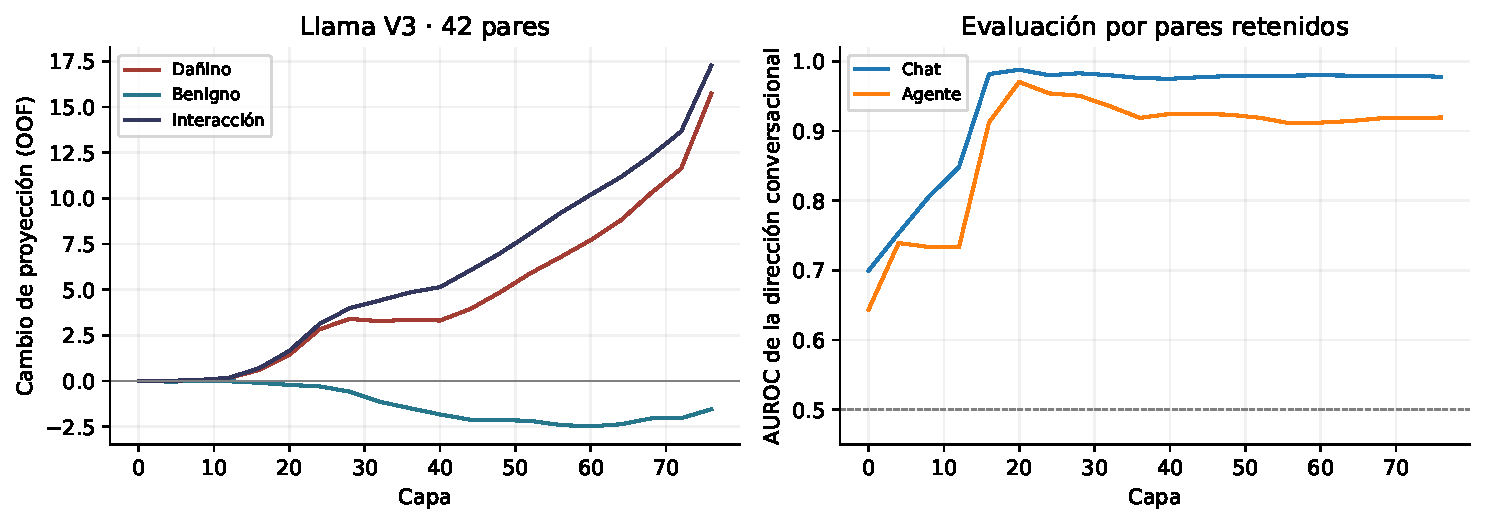
\includegraphics[width=0.94\textwidth]{avance_llama_capas}
\caption{Llama V3 sobre 42 pares. Izquierda: desplazamientos e interacción con direcciones cross-fit. Derecha: AUROC fuera de muestra de la dirección conversacional. Cada capa es una medición correlacionada del mismo corpus.}\label{fig:auroc_capa}\end{figure}

\subsection{Desplazamiento y control benigno}
\label{sec:desplazamiento}

El resultado central se expresa mediante cambios intra-par. Una proyección menor no demuestra por sí sola menor rechazo: es una medida geométrica. El brazo benigno permite descartar un desplazamiento idéntico de ambas clases sobre el eje, pero no identifica por sí solo el mecanismo completo ni elimina toda posible interacción de longitud y contenido.
\begin{table}[htbp]\centering\small
\begin{adjustbox}{max width=\textwidth}
\begin{tabular}{@{}lrrrr@{}}\toprule
Modelo & $\Delta p_h$ & $\Delta p_b$ & $\Delta^2p$ & IC 95\,\% interacción \\\midrule
Llama V3 & 15{,}7244 & -1{,}5438 & 17{,}2682 & $[14{,}9074;\ 19{,}4547]$ \\
Mistral V3 & 7{,}8359 & -0{,}5818 & 8{,}4178 & $[7{,}0992;\ 9{,}6758]$ \\
\bottomrule\end{tabular}\end{adjustbox}
\caption{Desplazamiento fuera de muestra, con dirección reajustada por fold. La interacción respeta el pareado dañino--benigno. Las unidades crudas no se comparan entre modelos.}\label{tab:gap}\end{table}

Las interacciones retenidas son positivas y sus intervalos excluyen cero. El test intra-par guardado reporta $p\simeq 10^{-4}$ en ambos casos, a la resolución de 10.000 permutaciones. La fracción común es aproximadamente $-9{,}8\,\%$ en Llama y $-7{,}4\,\%$ en Mistral. En ambos, el cambio benigno es pequeño frente al dañino y su contraste individual no permite afirmar un movimiento benigno distinto de cero al nivel $0{,}05$. La evidencia se concentra en el contraste entre brazos, no en declarar ausencia exacta de efecto en el benigno.

\subsection{Escala del efecto}
\label{sec:escala}

La separación cruda mezcla capacidad discriminativa y escala de proyección. En Llama, fuera de muestra, su pérdida es $82{,}6\,\%$, mientras la separación estandarizada cae $43{,}7\,\%$ y el AUROC pierde $0{,}0584$. En Mistral las pérdidas impresas son $84{,}7\,\%$, $63{,}8\,\%$ y $0{,}1627$, respectivamente. Ninguna cifra cruda debe presentarse como porcentaje de pérdida de seguridad.
\begin{table}[htbp]\centering\small
\begin{adjustbox}{max width=\textwidth}
\begin{tabular}{@{}lrrrr@{}}\toprule
Modelo & $d_{\rm chat}$ & $d_{\rm ag}$ & Pérdida en $d$ & $\kappa$ \\\midrule
Llama V3 & 3{,}2051 & 1{,}8036 & 43{,}7\,\% & 0{,}309 \\
Mistral V3 & 2{,}5289 & 0{,}9163 & 63{,}8\,\% & 0{,}422 \\
\bottomrule\end{tabular}\end{adjustbox}
\caption{Separación entre clases en unidades estandarizadas, obtenida sobre puntajes fuera de muestra. Estos valores de $d$ difieren del tamaño pareado del cambio de formato.}\label{tab:escala}\end{table}

\subsection{Comportamiento por explicitud}
\label{sec:estratos}

El análisis disponible utiliza los estratos originales de 18, 14 y 10 pares. El corpus ampliado cuenta con 42, 24 y 30, pero esos tamaños no se transfieren a las estimaciones siguientes.
\begin{table}[htbp]\centering\small
\begin{adjustbox}{max width=\textwidth}
\begin{tabular}{@{}llrrrr@{}}\toprule
Modelo & Estrato & Pares & Chat & Agente & Pérdida \\\midrule
Llama V3 & Explícito & 18 & 0{,}9907 & 0{,}9290 & 0{,}0617 \\
Llama V3 & Contextual & 14 & 0{,}9847 & 0{,}9643 & 0{,}0204 \\
Llama V3 & Apariencia legítima & 10 & 0{,}9400 & 0{,}8900 & 0{,}0500 \\
Mistral V3 & Explícito & 18 & 0{,}9722 & 0{,}8827 & 0{,}0895 \\
Mistral V3 & Contextual & 14 & 0{,}9439 & 0{,}7398 & 0{,}2041 \\
Mistral V3 & Apariencia legítima & 10 & 0{,}9000 & 0{,}7100 & 0{,}1900 \\
\bottomrule\end{tabular}\end{adjustbox}
\caption{AUROC por explicitud sobre puntajes fuera de muestra. El pequeño tamaño de los estratos y la ausencia de intervalos por estrato impiden establecer una ordenación poblacional firme.}\label{tab:estratos}\end{table}

La pérdida puntual máxima de Llama aparece en el estrato explícito y la de Mistral en el contextual. Por tanto, no hay una jerarquía universal de degradación según explicitud en estas ejecuciones. El estrato de apariencia legítima conserva señal por encima del azar en ambos modelos, pero no se interpreta como garantía de detección de solicitudes encubiertas nuevas.
\begin{figure}[htbp]\centering
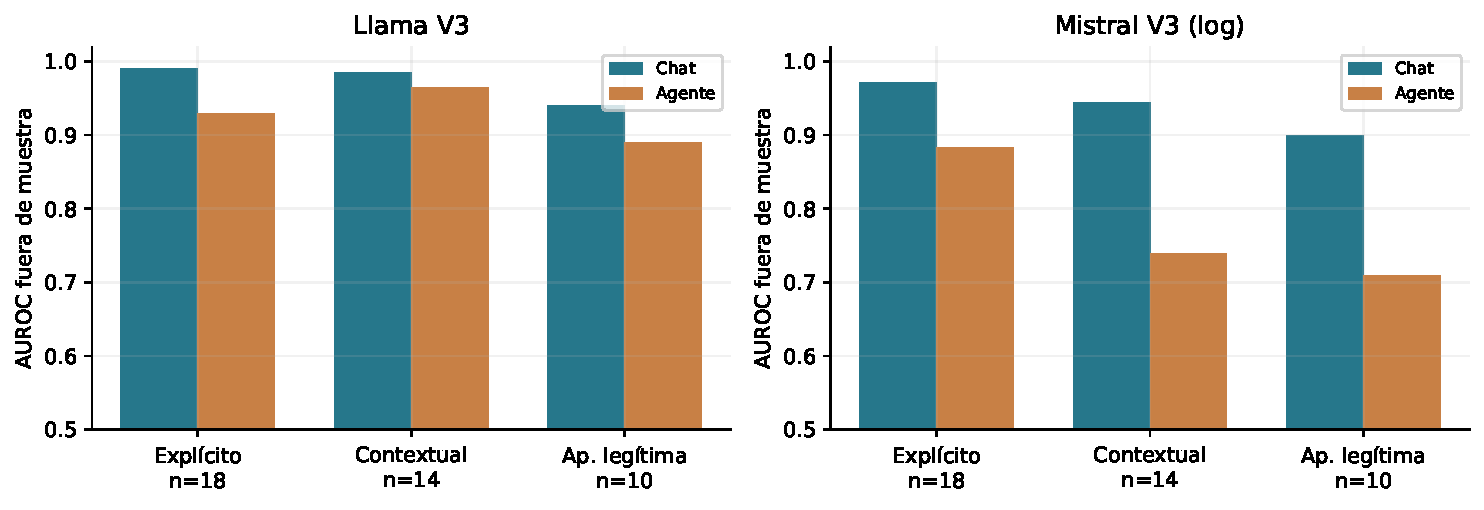
\includegraphics[width=0.94\textwidth]{avance_estratos}
\caption{Discriminación por explicitud en las dos ejecuciones principales. Ambas usan 42 pares; las barras son estimaciones puntuales, no diferencias estadísticamente contrastadas entre modelos.}\label{fig:cmp_estratos}\end{figure}

\subsection{Reorientación y monitores por estimador}
\label{sec:rotacion}

En Llama, capa 76, el coseno de muestra completa entre direcciones de medias es $0{,}2128$. Las fiabilidades entre mitades disjuntas son $0{,}9010$ en chat y $0{,}9220$ en agente. La estimación normalizada por el techo de fiabilidad da coseno $0{,}2204$ y ángulo descriptivo de unos $77^\circ$. La alineación es baja, pero no corresponde al coseno $0{,}051$ que la versión anterior atribuía a ese modelo.

La comparación logística produce coseno de muestra completa $0{,}0744$ y fiabilidades mucho menores, $0{,}2522$ y $0{,}2832$. Esa menor reproducibilidad obliga a interpretar con más cautela el ángulo. Las dos medidas no se promedian ni se sustituyen una por otra.
\begin{figure}[htbp]\centering
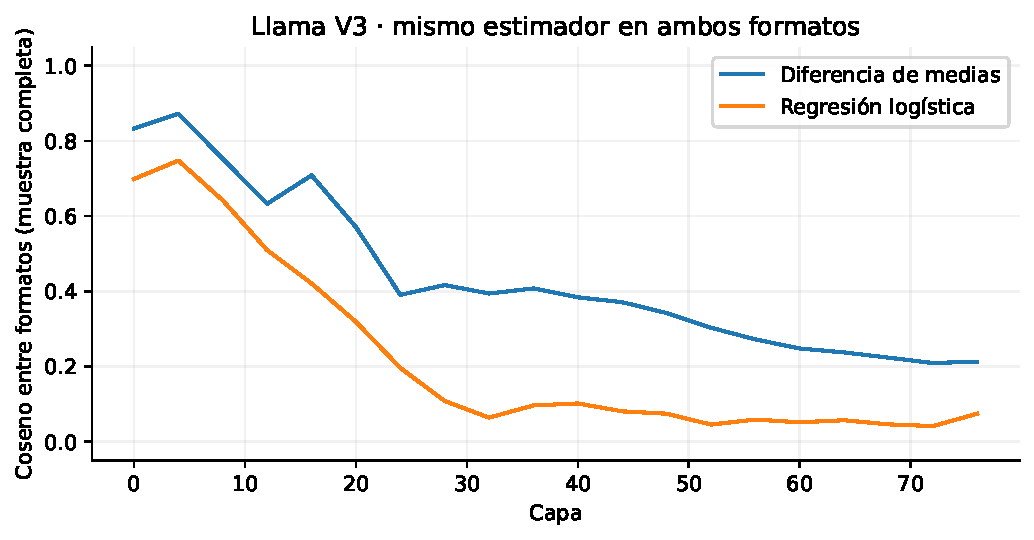
\includegraphics[width=0.94\textwidth]{avance_rotacion}
\caption{Llama V3: cosenos de muestra completa entre formatos, usando el mismo estimador en ambos. Los valores no son una prueba causal y deben leerse junto con la fiabilidad descrita en el texto.}\label{fig:cmp_rotacion}\end{figure}
\begin{table}[htbp]\centering\small
\begin{adjustbox}{max width=\textwidth}
\begin{tabular}{@{}lrrr@{}}\toprule
Modelo / estimador & AUROC OOF & $F_1$ OOF & FPR OOF \\\midrule
Llama / medias & 0{,}9707 & 0{,}8434 & 0{,}1429 \\
Llama / logística & 0{,}9926 & 0{,}9367 & 0{,}0000 \\
Mistral / logística (log) & 0{,}9347 & 0{,}8250 & 0{,}1190 \\
\bottomrule\end{tabular}\end{adjustbox}
\caption{Monitores agénticos evaluados por cinco folds. En Llama se usa capa 76; en Mistral, capa 30. El AUROC corresponde a la media de folds y $F_1$ al protocolo de umbrales retenidos; las métricas no son intercambiables.}\label{tab:monitores}\end{table}

El cero de falsos positivos de la logística de Llama corresponde a 42 benignos de este corpus. No demuestra una tasa poblacional nula ni seguridad de despliegue. La señal agéntica es aprovechable por un monitor ajustado en ese formato; eso no demuestra que el mecanismo interno de rechazo use espontáneamente el mismo eje.

\section{Evaluación y validación}
\label{sec:evaluacion-resultados}
\subsection{PCA del contraste conversacional}

PCA se ajusta sobre activaciones conversacionales concatenadas y centradas globalmente, según el procedimiento de métodos. La Tabla~\ref{tab:pca} incorpora los resultados que faltaban en la versión anterior. Los de Llama se comprobaron además desde las activaciones guardadas mediante el autovector principal de la matriz de Gram.
\begin{table}[htbp]\centering\small
\begin{adjustbox}{max width=\textwidth}
\begin{tabular}{@{}lrrr@{}}\toprule
Modelo & Capa & $|\cos(\mathrm{PC1},\hat{\bm{r}})|$ & Varianza de PC1 \\\midrule
Llama V3 & 28 & 0{,}9934 & 36{,}53\,\% \\
Llama V3 & 56 & 0{,}9936 & 25{,}91\,\% \\
Llama V3 & 76 & 0{,}9894 & 20{,}13\,\% \\
Mistral V3 & 18 & 0{,}968 & 30{,}3\,\% \\
Mistral V3 & 30 & 0{,}952 & 28{,}7\,\% \\
\bottomrule\end{tabular}\end{adjustbox}
\caption{Validación geométrica descriptiva, dentro de muestra. La alineación con PC1 no sustituye la evaluación fuera de muestra del AUROC.}\label{tab:pca}\end{table}
\begin{figure}[htbp]\centering
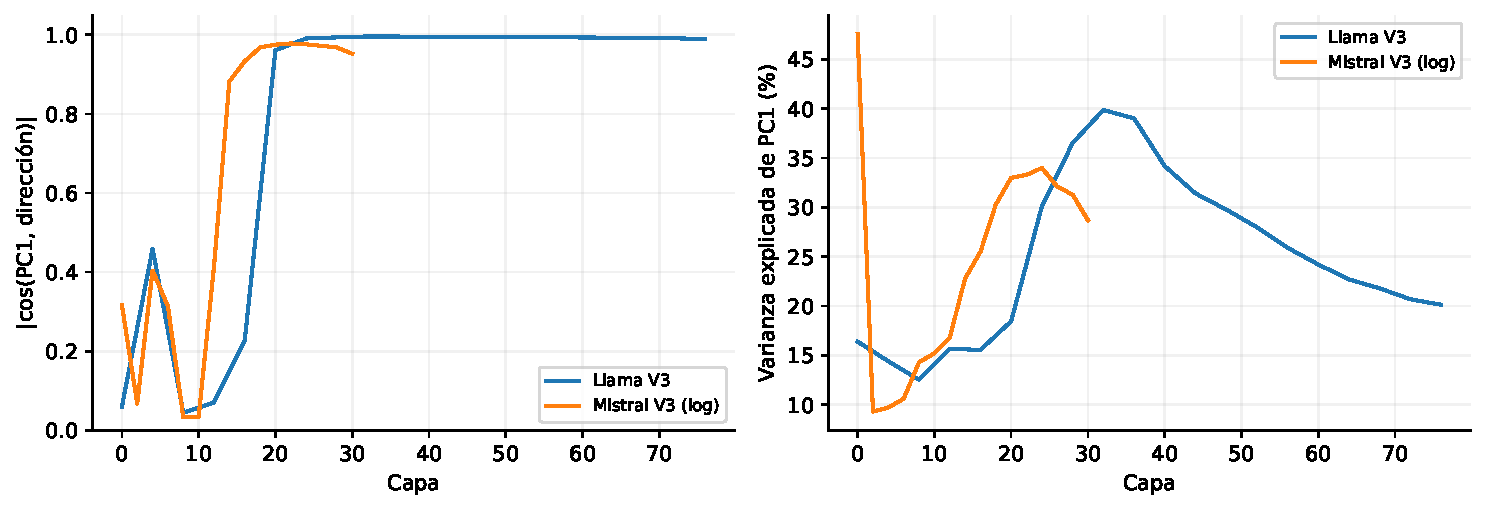
\includegraphics[width=0.94\textwidth]{avance_pca}
\caption{Alineación de PC1 y proporción de varianza explicada a lo largo de las capas. Las posiciones de capa son propias de cada arquitectura y los puntos de Mistral conservan la precisión impresa del log.}\label{fig:pca}\end{figure}

En capas iniciales el contraste no siempre coincide con PC1. En las capas profundas mostradas sí presenta alineación elevada, sin que PC1 explique toda la varianza: por ejemplo, en la capa 76 de Llama explica $20{,}13\,\%$. Este resultado respalda una estructura geométrica dominante de la muestra en esas capas, no la identidad entre un componente principal y una causa del rechazo.

\subsection{Circularidad y selección de capa}

En Llama, capa 76, el desplazamiento ingenuo es $16{,}2776$ y el cross-fit es $15{,}7244$: la diferencia equivale al $3{,}5\,\%$ del valor corregido. En Mistral, capa 30, pasa de $8{,}0227$ a $7{,}8359$, un $2{,}4\,\%$. La corrección reduce el efecto y este conserva su signo. Los conteos cross-fit son 42/42 y 39/42 decrecientes, respectivamente; constituyen una comprobación descriptiva sobre el corpus completo.

Para evitar reutilizar los pares que seleccionan una capa, la inferencia separada utiliza solo la otra mitad. La Tabla~\ref{tab:seleccion} resuelve la ambigüedad del conteo antiguo de 39/42: no debe presentarse como un conteo exclusivo de inferencia.
\begin{table}[htbp]\centering\small
\begin{adjustbox}{max width=\textwidth}
\begin{tabular}{@{}lrrrrr@{}}\toprule
Modelo & Selección & Inferencia & Capa & Decrecen & $\Delta p$ inferencia \\\midrule
Llama V3 & 21 & 21 & 76 & 21/21 & 16{,}5899 \\
Mistral V3 & 21 & 21 & 30 & 19/21 & 7{,}6873 \\
\bottomrule\end{tabular}\end{adjustbox}
\caption{Selección e inferencia sobre mitades disjuntas de pares. Los 42/42 o 39/42 del cross-fitting global no son el denominador de esta prueba.}\label{tab:seleccion}\end{table}

El intervalo de inferencia de Llama es $[14{,}0276;\ 18{,}9079]$ y el de Mistral $[6{,}0074;\ 9{,}1634]$. Sus pruebas de signos arrojan aproximadamente $9{,}54\times10^{-7}$ y $2{,}21\times10^{-4}$; ambas quedan bajo los umbrales Bonferroni $0{,}0025$ y $0{,}003125$. Sobre 200 particiones aleatorias, cada ejecución selecciona su misma capa en el $100\,\%$ de los casos guardados. Estas particiones describen estabilidad sobre el corpus observado; no multiplican el tamaño de muestra.

La prueba de signos depende de la dirección utilizada. Su invariancia se limita a reescalados positivos, no a cambios del eje. La separación entre ajuste y evaluación protege frente a circularidad, sin eliminar todos los supuestos de muestreo.

\section{Ensayos conductuales e intervención exploratoria}
\label{sec:conductual}

Llama V3 conserva las generaciones y sus etiquetas heurísticas. En solicitudes dañinas, el rechazo sin intervención pasa de 38/42 en chat ($90{,}5\,\%$) a 23/42 en agente ($54{,}8\,\%$). Dieciséis pares dejan de rechazar y uno cambia en sentido contrario, con McNemar exacto $p=0{,}000275$. En benignos las tasas son 5/42 y 1/42. Estas etiquetas describen respuestas generadas, no ejecución de tareas mediante herramientas, y su auditoría humana está pendiente.

Como ejemplo de intervención se reporta la capa 56, declarada explícitamente en la configuración de ese ensayo; es distinta de la capa 76 usada para el diagnóstico principal. Se evalúan 19 dañinos y 41 benignos que inicialmente no eran rechazados en formato agéntico.
\begin{table}[htbp]\centering\small
\begin{adjustbox}{max width=\textwidth}
\begin{tabular}{@{}lrrr@{}}\toprule
Dosis & Rechazo dañino & Control aleatorio & Rechazo benigno \\\midrule
0{,}5 & 6/19 & 1/19 & 0/41 \\
1{,}0 & 12/19 & 1/19 & 5/41 \\
2{,}0 & 19/19 & 1/19 & 40/41 \\
4{,}0 & 19/19 & 1/19 & 33/41 \\
\bottomrule\end{tabular}\end{adjustbox}
\caption{Llama V3, intervención exploratoria en capa 56. El control aleatorio tiene igual norma. Los denominadores corresponden a subconjuntos que no rechazaban inicialmente; no son los 42 pares completos.}\label{tab:causal}\end{table}
\begin{figure}[htbp]\centering
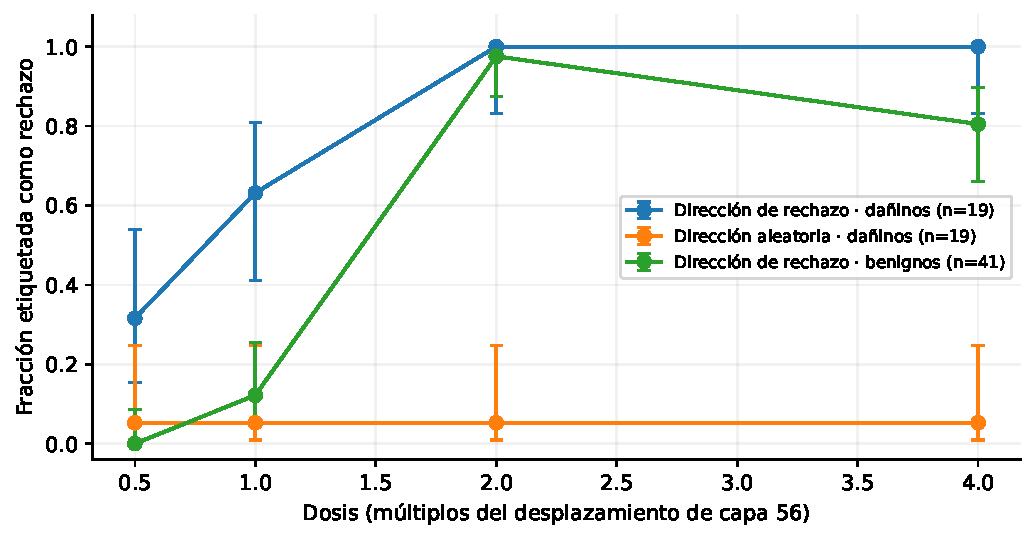
\includegraphics[width=0.94\textwidth]{avance_intervencion}
\caption{Respuesta a la dosis en capa 56. Barras: intervalos binomiales guardados. Una dosis que induce rechazo también en benignos no constituye una reparación selectiva.}\label{fig:causal}\end{figure}

En dosis 1 el rechazo dañino es 12/19 con dirección de rechazo y 1/19 con control aleatorio; McNemar pareado $p=0{,}000977$. El brazo benigno rechaza 5/41. En dosis 2 el rechazo dañino alcanza 19/19, pero también 40/41 benignos. El ensayo apoya un efecto de la adición sobre la conducta etiquetada en estas condiciones y muestra un costo de sobrerrechazo. No demuestra que la reorientación observada explique por sí sola el fallo ni resuelve la calibración de una defensa. Los valores $p$ por dosis son exploratorios y no están corregidos por todos los contrastes de capas y dosis.

Mistral conserva una línea base impresa de 19/42 rechazos dañinos en chat y 5/42 en agente, con McNemar $p\simeq0{,}0013$. Su registro termina durante la intervención; por ello no se presenta una curva causal completa ni se infiere su desenlace.

\section{Evidencia exploratoria de Qwen}

Los JSON históricos de Qwen usan igualmente 42 pares. En Qwen3-8B, capa 32, el AUROC held-out de la dirección conversacional es $0{,}5176$ en chat y $0{,}5108$ en agente: esta ejecución no establece una línea base discriminativa suficiente en esa capa. En Qwen3-32B, capa 46, los valores son $0{,}9694$ y $0{,}9558$. La configuración exportada es menos completa y no acredita todos los controles actuales. Se conservan como antecedentes experimentales, sin utilizarlos para sostener una réplica uniforme entre familias ni una ley de escala. Repetirlos con la versión corregida y el corpus ampliado es parte del trabajo pendiente.
                   % 4. Resultados y evaluación
\chapter{Discusión}
\label{chap:discusion}
\section{Síntesis de los avances}

El avance principal es haber convertido una comparación de proyecciones en un diagnóstico con controles explícitos. El contenido se conserva entre formatos, el brazo benigno distingue cambios comunes de contrastes específicos del daño y la evaluación por pares retenidos evita confundir separación de entrenamiento con generalización. La integración de PCA y la separación de selección e inferencia permiten responder a las observaciones sobre validación geométrica y reutilización de la muestra.

Los resultados de Llama V3 y el registro de Mistral V3 sostienen una reducción del margen discriminativo sobre la dirección conversacional. En ambos, la interacción sigue siendo positiva fuera de muestra y el AUROC agéntico se mantiene por encima del azar. Por tanto, los datos disponibles describen una degradación de margen, con intensidad dependiente del modelo, y no una desaparición completa de información discriminativa.

\section{Interpretación del cambio de representación}

La contracción de escala explica parte de la gran caída de separación cruda. La pérdida persiste en unidades estandarizadas y en AUROC, por lo que no se agota en un cambio de unidades. Sin embargo, restar el control benigno tampoco convierte automáticamente el resto en una medida de rechazo: la etiqueta dañino--benigno, la proyección y la decisión conductual son tres objetos distintos.

La baja alineación entre direcciones comparables en Llama es compatible con una reorientación del contraste entre clases. La fiabilidad alta de las direcciones de medias vuelve esa descripción más interpretable que un coseno obtenido de sondas poco reproducibles. Un monitor agéntico logra recuperar parte de la señal, pero su existencia no prueba que el modelo use ese eje para decidir. El comportamiento puede depender de otras direcciones, capas y transformaciones posteriores.

La comparación entre modelos tampoco aísla el número de parámetros. Cambian arquitectura, entrenamiento, plantilla y distribución de proyecciones. Las diferencias puntuales entre Llama y Mistral no permiten concluir que aumentar tamaño preserve la seguridad. Las ejecuciones históricas de Qwen refuerzan la necesidad de revisar cada configuración y de no seleccionar solo resultados favorables.

\section{Lo que aporta la intervención}

El ensayo complementario de Llama permite ir más allá de asociar dos cantidades: añadir activación en una dirección cambia la fracción de respuestas etiquetadas como rechazo respecto de un control aleatorio. Su interpretación se limita a esa manipulación y a los subconjuntos ensayados. No demuestra necesidad del mecanismo ni que la rotación sea el mediador del efecto del formato. El rechazo masivo de benignos a dosis altas descarta interpretar cualquier incremento de rechazo como una mejora selectiva de seguridad.

La heurística de etiquetado hace auditables los cálculos, pero puede confundir una negativa superficial, un rechazo seguido de información o una respuesta que aparenta usar herramientas. La lectura humana independiente de las generaciones es necesaria antes de elevar estos resultados a una conclusión conductual firme. En Mistral la evidencia causal local es incompleta.

\section{Limitaciones y alcance de validez}

La primera limitación es muestral: el corpus construido tiene 96 pares, mientras las ejecuciones analizadas usan 42 y el estrato más pequeño solo diez. Las cuatro variantes, las capas y los 200 splits no son nuevas unidades independientes. La anotación de explicitud no dispone todavía de una segunda clasificación independiente para estimar acuerdo.

La segunda es el alcance del formato. Se describe capacidad de usar herramientas mediante un mensaje y esquemas simulados; no se observa una tarea autónoma ejecutada durante varios pasos. El contraste principal cambia sistema y herramientas conjuntamente. La interacción con el brazo benigno no descarta por completo efectos de longitud, delimitadores o interacciones entre esos componentes y el contenido.

La tercera es la inferencia. El cross-fitting controla reutilización de cada par, pero induce dependencia por entrenamiento compartido. Los intervalos de los puntajes guardados no incorporan toda la incertidumbre de volver a ajustar el pipeline. La inferencia sobre mitades disjuntas reduce el sesgo de selección, pero evalúa solo 21 pares. Los ángulos ajustados por fiabilidad son estimaciones bajo supuestos, no constantes conocidas.

La cuarta es de reproducibilidad. La copia de activaciones y la duplicación de tokens especiales exigieron correcciones. Las cifras de versiones distintas deben permanecer identificadas; no se atribuye su diferencia a fluctuación de muestreo sin comprobar la implementación. Llama V3 ofrece activaciones y resultados estructurados; Mistral V3 solo está disponible como registro redondeado. Los monitores carecen de evaluación externa y sus umbrales pueden no transferirse a otro corpus o despliegue.

\section{Implicaciones para el avance siguiente}

El siguiente paso informativo es repetir el protocolo corregido sobre los 96 pares construidos, con la misma versión de código, configuración exportada y conservación de activaciones y generaciones. Debe fijarse un protocolo de comparación entre modelos y estimadores, reservar evaluación independiente de umbrales e incorporar una segunda anotación. En paralelo, el análisis factorial puede separar mensaje de sistema y herramientas, con controles de longitud y de plantilla. Solo después corresponde valorar una defensa operacional.
                   % 5. Discusión
\chapter{Conclusiones y recomendaciones del avance}
\label{chap:conclusiones}
\section{Conclusiones}

Se construyó y verificó un corpus contrastivo ampliado de 96 pares, con cuatro variantes por par y control de identidad de texto y simetría del andamiaje. Ese es un resultado de construcción de datos. Las conclusiones experimentales de esta versión se refieren a las ejecuciones disponibles de 42 pares y no se extrapolan como si provinieran del corpus ampliado.

En Llama V3 y Mistral V3, la dirección conversacional conserva capacidad discriminativa en formato agéntico, aunque con menor margen: el AUROC fuera de muestra pasa de $0{,}9779$ a $0{,}9195$ en Llama y de $0{,}9478$ a $0{,}7851$ en Mistral. La interacción con el control benigno y la pérdida estandarizada muestran que el resultado no se reduce a una traslación idéntica de ambas clases ni a un mero cambio de escala.

La validación geométrica muestra alineación elevada entre PC1 y la diferencia de medias en capas profundas, y Llama presenta baja alineación entre los contrastes de ambos formatos. La interpretación debe mantener separados diferencia de medias y regresión logística e incorporar la fiabilidad de sus direcciones. Estas observaciones caracterizan representaciones; no identifican por sí solas la causa general del fallo del rechazo.

La disponibilidad de monitores fuera de fold acredita una viabilidad preliminar de recuperar señal agéntica. El ensayo de intervención en Llama aporta evidencia exploratoria de que añadir activación puede aumentar el rechazo, con un costo creciente en solicitudes benignas. La calibración, la validación humana y la transferencia siguen abiertas. Las corridas históricas de Qwen no justifican afirmar un patrón uniforme en todas las familias.

\section{Aportes del trabajo hasta este corte}

El trabajo aporta un corpus ampliado auditable, un pipeline de extracción y análisis con controles de circularidad y pareado, resultados geométricos trazables para Llama y un registro de réplica en Mistral, además de ensayos conductuales conservados para auditoría. La separación entre unidades crudas, separación estandarizada y AUROC evita interpretar un cambio de escala como pérdida total de seguridad. La separación de selección e inferencia hace explícito qué pares sustentan cada contraste.

\section{Recomendaciones}

Se recomienda consolidar los artefactos completos de Mistral, ejecutar el corpus de 96 pares en los modelos con configuración común, documentar versiones y hashes y reservar datos para validación externa. Es necesario completar doble anotación de explicitud y revisión independiente de las generaciones, comparar formalmente estimadores sobre las mismas particiones y evaluar umbrales en condiciones distintas de aquellas que los ajustan. La extensión a trayectorias, autonomía y herramientas ejecutadas requiere un diseño adicional y no se considera validada por este avance.
                 % 6. Conclusiones y recomendaciones

% =============================================================
% GLOSARIO Y ANEXOS
% =============================================================

\clearpage
\pagestyle{plain}

\chapter*{Glosario de notación}
\addcontentsline{toc}{chapter}{Glosario de notación}

Se reúnen a continuación la notación y las medidas que aparecen en el capítulo de resultados, de modo que puedan consultarse sin volver sobre la formalización.

\begin{description}[leftmargin=0pt, labelwidth=0pt, labelsep=0pt, style=nextline, itemsep=0.45em]

  \item[Cono de influencia ($\mathcal{C}(i)$)] Conjunto de \textit{tokens} de la secuencia que pueden alterar la representación de la posición $i$. Por la máscara causal es $\{1, \dots, i\}$, de modo que la posición final del estímulo renderizado tiene acceso causal al estímulo completo, incluidos sus delimitadores. Es la razón por la que el estudio mide en esa posición.

  \item[Capa de referencia] Capa de cada modelo en la que el procedimiento maximiza el desplazamiento medido y sobre la que se reportan las cifras principales. En las ejecuciones principales de esta versión es 30 en Mistral V3 y 76 en Llama V3; las ejecuciones históricas se identifican por separado.

  \item[Índice de Jaccard ($J$)] Proporción de términos compartidos entre la rama dañina y la benigna de un par, sobre el total de términos distintos que usan ambas. Mide la simetría léxica del pareado: vale uno si las dos ramas usan el mismo vocabulario y cero si no comparten ninguno.

  \item[Proyección ($p$)] Medida geométrica de cuánto se alinea la representación de una instrucción con la dirección de rechazo. Un valor alto indica mayor alineación con ese eje, no que el modelo reconozca el peligro; su capacidad de separar instrucciones dañinas de benignas se cuantifica aparte, mediante el AUROC.

  \item[Gap de proyección ($\Delta p_{h}$)] Diferencia entre la proyección media de las instrucciones dañinas en formato conversacional y la de esas mismas instrucciones en formato agéntico. Mide en qué medida \emph{disminuye} esa alineación al cambiar de formato, y es el resultado central de este trabajo.

  \item[Interacción o diferencia en diferencias ($\Delta^{2} p$)] Diferencia entre el desplazamiento del brazo dañino y el del benigno. Es la parte del efecto específica del contenido dañino.

  \item[Fracción común ($\varphi$)] Proporción del desplazamiento dañino que el brazo benigno reproduce. Un valor negativo indica que los dos brazos se desplazan en sentidos opuestos.

  \item[AUROC] Probabilidad de que, tomadas al azar una instrucción dañina y una benigna, la dañina proyecte más que la benigna. Un valor de 1 indica separación perfecta y uno de 0{,}5 una separación equivalente al azar.

  \item[Gap de detección ($\Delta$AUROC)] Diferencia entre el AUROC del formato conversacional y el del agéntico. Es la diferencia neta de probabilidades de ordenación correcta; admite cambios en ambos sentidos y no cuenta exclusivamente los aciertos perdidos. Es una cantidad distinta del gap de proyección y responde a otra pregunta: aquel mide intensidad de la respuesta, este mide capacidad de discriminación.

  \item[Contracción de escala ($\kappa$)] Cociente entre la desviación estándar de las proyecciones en formato agéntico y la observada en formato conversacional. Cuantifica qué parte de una pérdida medida en unidades crudas corresponde a un cambio de unidades.

  \item[$\bm{w}_{\mathrm{DM}}$ y $\bm{w}_{\mathrm{LR}}$] Direcciones agénticas estimadas por diferencia de medias y regresión logística, respectivamente. Se reportan por separado. La primera es el contraste entre centroides dentro del formato agéntico. Su coseno con la dirección de rechazo conversacional mide cuánto ha rotado el eje sobre el que el modelo codifica la peligrosidad.

\end{description}

\clearpage

\appendix
\chapter{Trazabilidad y material complementario}
\label{app:trazabilidad}
\section{Corpus construido y muestra ejecutada}

El archivo \texttt{dataset\_v2.jsonl} contiene 96 pares, 384 entradas, 62 pares propios y 34 derivados de AgentHarm. El informe de construcción se adjunta en \texttt{evidencia/}. La identidad del texto entre formatos y la simetría de sistema, herramientas y esquemas dentro de cada formato se verificaron en 96/96 pares. Hay 64 herramientas distintas utilizadas. Los conteos por explicitud son 42, 24 y 30. El corpus original ejecutado tiene 42 pares, con estratos de 18, 14 y 10. Estos dos conjuntos no se intercambian al informar denominadores.

La revisión asistida de pares no sustituye una segunda anotación humana independiente. El cálculo de acuerdo entre anotadores permanece pendiente. Las etiquetas y el informe del corpus acompañan el material complementario; las instrucciones completas y las generaciones se conservan en el repositorio de investigación y no se reproducen aquí como un catálogo de tareas.

\section{Configuración de la corrida principal}

Llama V3 emplea \texttt{meta-llama/Llama-3.3-70B-Instruct}, precisión FP16, semilla 42, cinco folds, diez repeticiones de la sonda lineal, una de MLP, diez controles permutados, 10.000 remuestreos y 200 divisiones de selección. El barrido usa capas 0, 4, 8, hasta 76. El corpus se carga por la opción predeterminada original, con \texttt{dataset\_path=null}; las activaciones y sus metadatos identifican 42 pares. Las intervenciones declaradas son en capas 56, 52 y 28, con dosis 0,5; 1; 2 y 4 y un máximo de 64 tokens nuevos.

La configuración exportada de Mistral declara FP16, barrido de 16 capas y 42 pares. Su registro contiene PCA, evaluación retenida y selección de capa, pero el archivo termina durante la etapa causal. La ausencia local del JSON y de sus activaciones limita la reproducción de ese análisis. Los resultados redondeados se identifican como tales.

\section{Control de versiones de resultados}

La versión anterior de la tesis empleaba para Llama la capa 56 y $\Delta p\simeq5{,}74$. Esta versión utiliza Llama V3, capa 76, y reporta como principal el valor fuera de muestra $15{,}7244$. El código documenta la sustitución de una copia asíncrona GPU--CPU por una bloqueante y la corrección de duplicación de BOS. Por eso las diferencias entre ejecuciones no se interpretan como fluctuación estadística sin verificar implementación. El repositorio conserva las corridas anteriores para inspección; sus cifras no se mezclan con V3.

Los archivos de evidencia adjuntos incluyen métricas extraídas y un manifiesto SHA-256 de las fuentes originales. El hash identifica el contenido revisado, pero no reconstruye una revisión de código de entrenamiento ni certifica una ejecución externa que no esté archivada. La regeneración de tablas y figuras se realiza con \texttt{scripts/actualizar\_tesis\_avances.py}, incluido también como \texttt{regenerar\_avances.py} en este paquete, para ejecutarse desde el repositorio original con sus resultados.

\section{Estado de las observaciones del tutor}

Se actualizaron resumen y abstract; se definieron los conceptos desde la introducción; se precisó el formato como sistema y herramientas; se verificó simetría entre ramas; se documentó autoría y apoyo de anotación; se distinguió proyección de rechazo; se incorporaron PCA y su procedimiento; se corrigió la interpretación de la prueba de signos; se separaron selección e inferencia y se retiró cualquier equivalencia inferida solo de cercanía entre sonda y MLP. También se añadieron discusión, conclusiones del avance y este material complementario.

La revisión ortográfica normaliza los demostrativos del texto editado. No se dispone de la nota original para certificar el fragmento concreto señalado por el tutor. La recomendación de retroalimentación externa es de proceso y no se marca como realizada a partir de los archivos. La réplica de 96 pares, la segunda anotación, la auditoría humana conductual y la validación externa permanecen abiertas.

\section{Guion breve para presentar el avance}

La presentación puede organizarse en seis pasos: problema y pregunta; diseño pareado y corpus ampliado construido; evidencia ejecutada sobre 42 pares; pérdida de margen y control benigno; validación con PCA, cross-fitting y selección separada; e intervención exploratoria, limitaciones y siguiente ejecución. En cada diapositiva de resultados debe indicarse modelo, capa, estimador y denominador. Las figuras de esta versión están disponibles en PDF y PNG y pueden reutilizarse directamente.


% =============================================================
% REFERENCIAS
% =============================================================

\clearpage
\chapter*{Referencias}
\addcontentsline{toc}{chapter}{Referencias}
\printbibliography[heading=none]

\end{document}
